\documentclass{article}

% if you need to pass options to natbib, use, e.g.:
\PassOptionsToPackage{numbers, compress}{natbib}

 \usepackage[main, final]{neurips_2026}

% "preprint" option is used for arXiv or other preprint submissions
 % \usepackage[preprint]{neurips_2026}

% to avoid loading the natbib package, add option nonatbib:
%    \usepackage[nonatbib]{neurips_2026}

\usepackage[utf8]{inputenc} % allow utf-8 input
\usepackage[T1]{fontenc}    % use 8-bit T1 fonts
\usepackage{hyperref}       % hyperlinks
\usepackage{url}            % simple URL typesetting
\usepackage{booktabs}       % professional-quality tables
\usepackage{amsfonts}       % blackboard math symbols
\usepackage{nicefrac}       % compact symbols for 1/2, etc.
\usepackage{microtype}      % microtypography
\usepackage{xcolor}         % colors
\usepackage[dvipsnames]{xcolor}
\usepackage{amsmath}
\usepackage{amsthm}
\usepackage{amssymb}
\usepackage{bm}
\usepackage{graphicx}
\usepackage{cleveref}
\crefname{figure}{Figure}{Figures}
\Crefname{figure}{Figure}{Figures}
\usepackage{inconsolata}
\newtheorem{proposition}{Proposition}
\usepackage{natbib}
\usepackage{etoolbox}
\usepackage{array}
% \usepackage{framed}
\usepackage{tcolorbox}
\tcbuselibrary{breakable}
% Note. For the workshop paper template, both \title{} and \workshoptitle{} are required, with the former indicating the paper title shown in the title and the latter indicating the workshop title displayed in the footnote. 
% \title{Jacobian Scopes: A Unified Geometric Framework for Token-Level LLM Attributions}
\title{Jacobian Scopes: A Unified Geometric Framework for Token-Level LLM Attribution}


\author{%
  \textbf{Toni J.B. Liu}\textsuperscript{$\spadesuit$},\,
  \textbf{Baran Zadeoğlu}\textsuperscript{$\spadesuit$},\,
  \textbf{Gurbir Arora}\textsuperscript{$\spadesuit$},\,
  \\
  \textbf{Raphaël Sarfati}\textsuperscript{$\spadesuit\,\diamondsuit$},\,
  \textbf{Nicolas Boullé}\textsuperscript{$\heartsuit$},\,
  \textbf{Christopher J. Earls}\textsuperscript{$\spadesuit$}
\\
  \textsuperscript{$\spadesuit$}Cornell University, USA,\,
  \textsuperscript{$\heartsuit$}Imperial College London, UK, \,
  \textsuperscript{$\diamondsuit$}Goodfire AI, USA
\\
  \small{
    \textbf{Correspondence:} \href{mailto:jl3499@cornell.edu}{jl3499@cornell.edu}
  }
}


\begin{document}


\maketitle
\begin{abstract}
Large language models (LLMs) make next-token predictions based on clues present in their
context, such as semantic descriptions and in-context examples. Yet, elucidating which prior
tokens most strongly influence a given prediction remains challenging due to the proliferation of layers and attention heads in modern
architectures. We propose \emph{Jacobian Scopes},
a suite of gradient-based, token-level causal
attribution methods for interpreting LLM predictions. Grounded in perturbation theory and
information geometry, Jacobian Scopes quantify how input tokens influence various aspects
of a model’s prediction, such as specific logits, the full predictive distribution, and model
uncertainty (effective temperature). Through
case studies spanning instruction understanding, translation, and in-context learning (ICL),
we demonstrate how Jacobian Scopes reveal
implicit political biases, uncover word- and
phrase-level translation strategies, and shed
light on recently debated mechanisms underlying in-context time-series forecasting.
On token-ablation faithfulness benchmarks (LAMBADA and IWSLT2017) across six LLMs, the distribution-level Fisher and Temperature Scopes significantly outperform established gradient-based attribution methods in 10 of 12 model--dataset settings.
To facilitate exploration of Jacobian Scopes on custom text, we open-source our implementations and provide a cloud-hosted interactive demo at \url{https://huggingface.co/spaces/Typony/JacobianScopes}.
\end{abstract}

% \begin{abstract}
% Gradient-based attribution methods for large language models (LLMs) have so far been limited to explaining scalar outputs --- the logit of a single target token.
% Yet LLM predictions are inherently distributional, and many practically important questions concern the full predictive distribution: which tokens make the model uncertain? Which drive a broad range of plausible continuations?
% We propose \emph{Jacobian Scopes}, a unified framework that fills this gap by projecting the input-to-output Jacobian onto different directions in output space via a single vector-Jacobian product, requiring only one backward pass.
% This yields three complementary methods: \textbf{Semantic Scope} attributes a specific target logit; \textbf{Fisher Scope}, grounded in information geometry, identifies tokens that most alter the overall shape of the predicted distribution; and \textbf{Temperature Scope} traces which tokens govern the model's predictive confidence.
% Fisher and Temperature Scopes are, to our knowledge, the first attribution methods to natively target distributional rather than pointwise features of LLM predictions.
% Through case studies spanning instruction following, translation, and in-context time-series forecasting, Jacobian Scopes reveal implicit political biases, uncover word- and phrase-level translation strategies, and illuminate the nearest-neighbor pattern-matching mechanisms underlying LLM forecasting.
% Quantitative evaluation on LAMBADA and IWSLT2017 across six leading LLMs (LLaMA-3.2, Qwen2.5, Gemma-3) confirms that Jacobian Scopes consistently match or outperform Input $\times$ Gradient and Integrated Gradients, at a fraction of the latter's computational cost.
% % To facilitate exploration of Jacobian Scopes on custom text, we open-source our implementations and provide a cloud-hosted interactive demo at \url{https://huggingface.co/spaces/Typony/JacobianScopes}.
% To facilitate exploration on custom text, we will open-source our implementations and provide a cloud-hosted interactive demo if the manuscript is accepted.
% \end{abstract}

\newcommand{\Toni}[1]{{\color{blue}{TL: #1}}}


\section{Introduction}
Large Language Models (LLMs) exhibit surprising emergent abilities, 
such as multi-step \cite{huang-chang-2023-towards} and in-context learning (ICL) \cite{dong-etal-2024-survey,garg2023transformerslearnincontextcase}.
However, the mechanistic underpinning of these emergent abilities remains a deep and open question \cite{olsson2022context,reddy2023mechanisticbasisdatadependence,von2023transformers}. 
This has fueled a growing endeavor, across academia and industry, 
to interpret and explain LLMs' inference process during such emergent thinking modes; 
as when writing \cite{wan2023kellywarmpersonjoseph,guo2024biaslargelanguagemodels} and reasoning \cite{wei2022chain, wang2023understandingchainofthoughtpromptingempirical}. 

In this work, we present a suite of gradient-based causal attribution methods called \emph{Jacobian Scopes}.
Jacobian Scopes explain LLM predictions in terms of influential input tokens.
This is achieved by analyzing the Jacobian matrix, which captures the locally linearized relation between
the predictive distribution and input embeddings.

Jacobian Scopes come in three variants: \textbf{Semantic}, \textbf{Fisher}, and \textbf{Temperature Scopes}, each corresponding to a different \emph{explanandum}, or attribution objective: logit of a certain token, the full predictive distribution, and the model's uncertainty (effective temperature). 
An overview of the framework is illustrated in \cref{fig:schematic}.

We showcase the efficacy of our proposed Jacobian Scopes through a range of case studies,
including natural language instruction such as system prompts and translation,
as well as ICL tasks such as 
time-series forecasting  \cite{gruver2024largelanguagemodelszeroshot,mirchandani2023largelanguagemodelsgeneral}.
We further evaluate attribution faithfulness quantitatively on two benchmark datasets (LAMBADA \cite{paperno-etal-2016-lambada} and IWSLT2017 \cite{cettolo-etal-2017-overview}) 
across three suites of leading LLMs: LLaMA-3.2 \cite{llama3-2024}, Qwen2.5 \cite{qwen2025qwen25} and Gemma-3 \cite{gemmateam2025gemma3technicalreport}.

\begin{figure}[t]
  \centering
  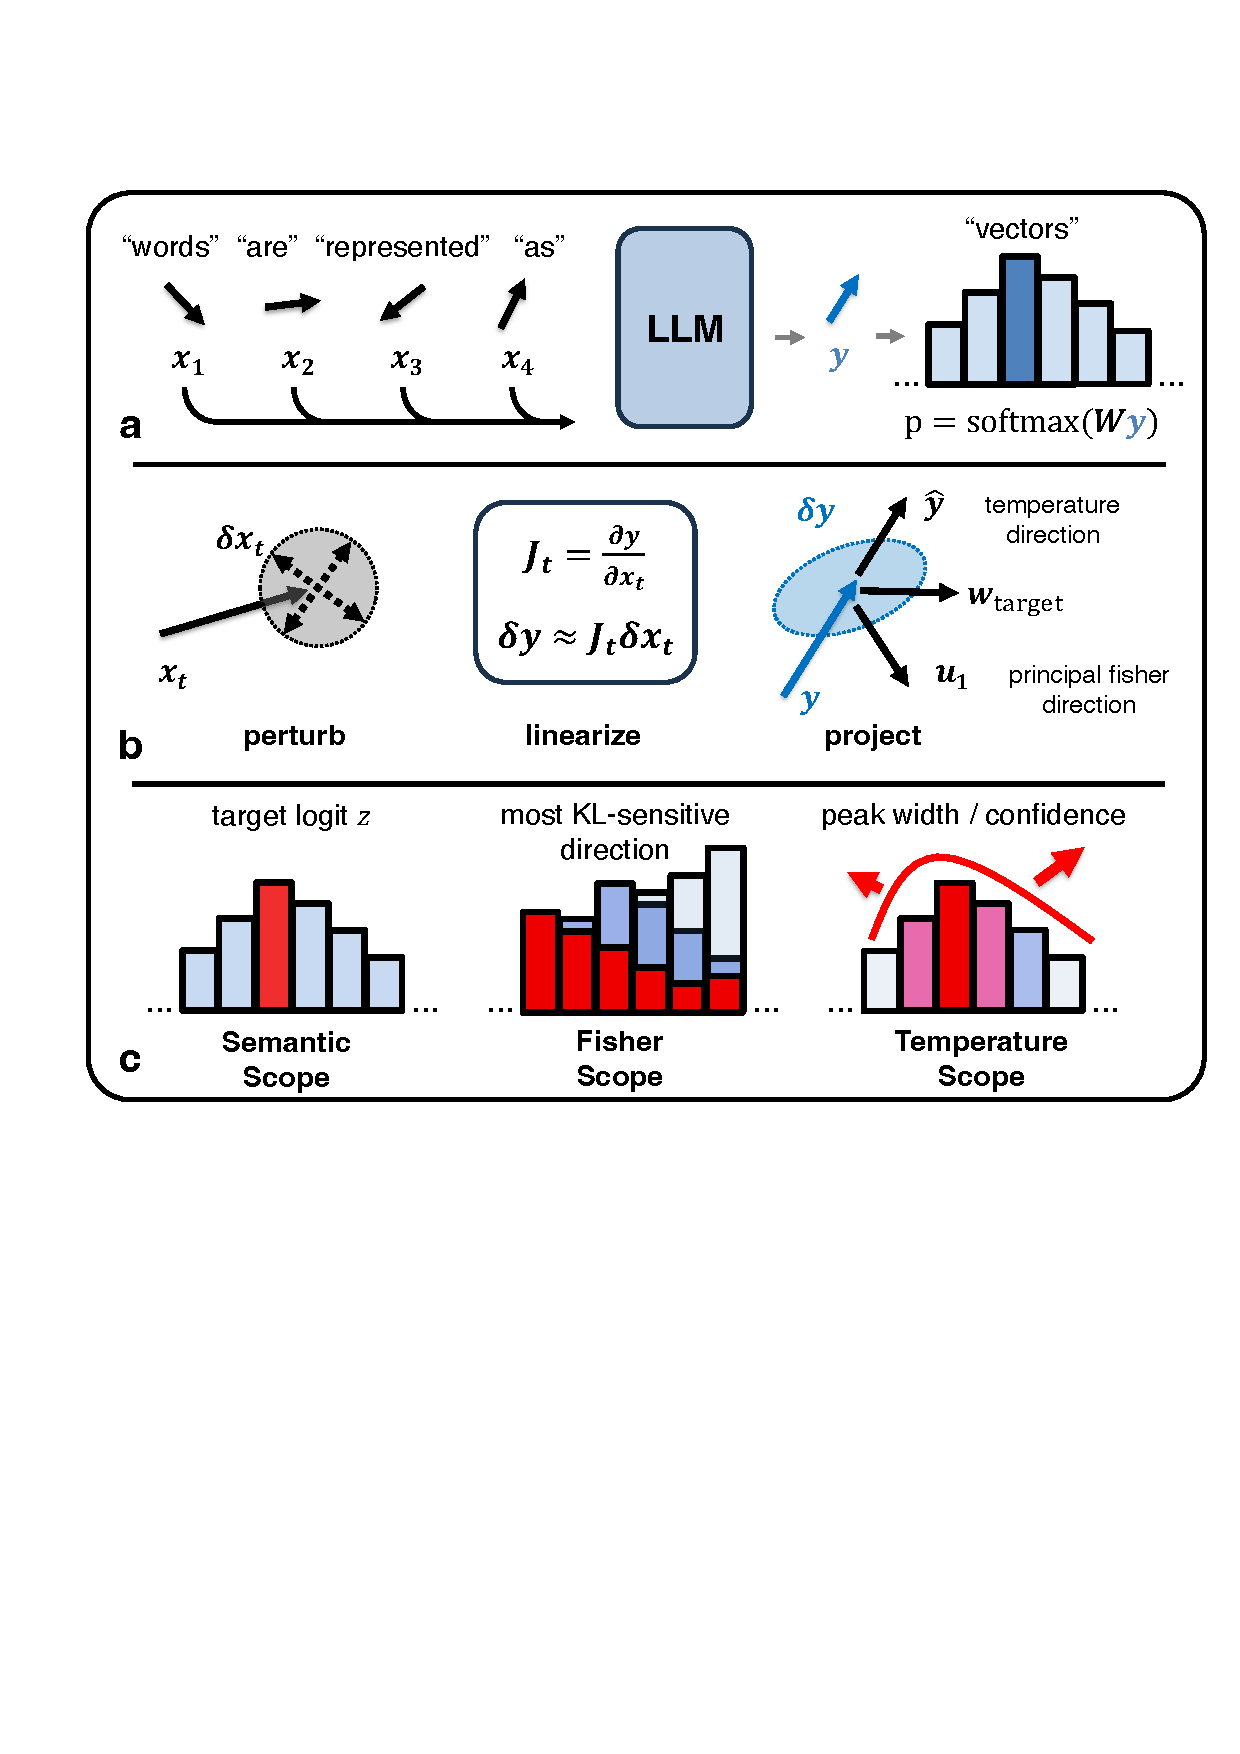
\includegraphics[width=1\textwidth]{figures/schematics.pdf}
  \caption{\textbf{Overview of Jacobian Scopes.}
  \textbf{(a)} An autoregressive LLM maps an input token sequence to a hidden state $\bm{y}$, which is decoded into a predictive distribution over the vocabulary.
  \textbf{(b)} A small perturbation to any input token is propagated to the output via the Jacobian $\bm{J}_t$, then projected onto a direction $\bm{v}$ in output space; the magnitude of this projection defines the token's influence score, computable in a single backward pass. The three Scopes correspond to $\bm{v} = \bm{w}_\mathrm{target}$ (target unembedding row), $\bm{v} = \bm{u}_1$ (principal Fisher direction), and $\bm{v} = \hat{\bm{y}}$ (normalized hidden state).
  \textbf{(c)} The three Jacobian Scope variants each target a different feature of the model's output: \textbf{Semantic Scope} asks which input tokens drive the predicted probability of a specific target word; \textbf{Fisher Scope} asks which tokens most change the overall shape of the predicted distribution; and \textbf{Temperature Scope} asks which tokens control the model's confidence, i.e., how sharply peaked the distribution is.}
  \label{fig:schematic}
\end{figure}

\section{Related work}
\label{sec:related_work}
Gradient-based attribution methods were first systematically developed for image classifiers.
\citet{simonyan2013deep} introduced class saliency maps by computing the
gradient of the predicted class score with respect to the input pixels,
identifying which image regions drive a given classification decision in a
single backward pass.
Building on this, \citet{shrikumar2017learning} proposed DeepLIFT, which
propagates neuron contribution scores by comparing each activation to a
reference state; gradient $\times$ input --- the elementwise product of the
input embedding and its gradient with respect to the target logit --- arises
as a simpler special case and serves as a baseline in our evaluations.
Grad-CAM \citep{Ramprasaath-Grad-Cam-2017} extends gradient saliency to produce spatially coarser but more semantically coherent maps by pooling gradients across feature channels.

A key challenge with plain gradient saliency is that the resulting maps are
often noisy and fail to sharply localize the relevant input features.
SmoothGrad \citep{smilkov2017smoothgradremovingnoiseadding} addresses this for
vision models by averaging sensitivity maps over many copies of the input
perturbed with Gaussian noise.
Integrated Gradients \citep{Sundararajan-Axiomatic-Attribution-DNN-2017}
instead eliminates path-dependence by integrating the gradient along a linear
interpolation from a null baseline to the actual input, satisfying axiomatic
desiderata such as Sensitivity and Implementation Invariance.
\citet{sanyal2021discretizedintegratedgradientsexplaining}
subsequently adapted this path integration to the discrete embedding space of
language models.
Outside the gradient paradigm, SHAP \citep{lundberg2017unified} provides model-agnostic attribution scores grounded in Shapley values from cooperative game theory, offering strong axiomatic guarantees but at combinatorial cost that must be approximated in practice.

A complementary line of work interprets transformers through the lens of attention weights.
\citet{Clark-Berts-Attention-2019} visualize BERT's attention patterns and identify heads that track syntactic and coreference relations.
\citet{abnar-zuidema-2020-quantifying} extend this with attention rollout and attention flow, which propagate attention weights across layers to produce more faithful input-attribution scores.
While intuitive and computationally cheap, these attention-based scores do not directly measure the causal influence of input tokens on model outputs, and can be misleading as attribution methods \citep{heimersheim2024useinterpretactivationpatching}.
\citet{ferrando-etal-2022-towards} address this for neural machine translation by proposing ALTI (Aggregated LaTent Interaction), a gradient-based method that attributes each generated target token to specific source tokens; our Fisher Scope case study on translation (\cref{fig:translating Dante}) can be viewed as a distributional generalization of this attribution objective.

More recently, mechanistic interpretability methods have sought to go beyond input-output sensitivity and trace computations through specific model circuits.
Activation patching \citep{heimersheim2024useinterpretactivationpatching, pmlr-v235-ghandeharioun24a} localizes responsible components by intervening on intermediate representations, while circuit tracing \citep{ameisen2025circuit} reconstructs full computational graphs.
Sparse autoencoder (SAE) probes \citep{lieberum2024gemmascopeopensparse} decompose residual stream activations into interpretable features.
These methods offer fine-grained mechanistic insights, but are substantially more expensive and architecture-specific than gradient-based approaches.

All gradient-based methods described above attribute a \emph{scalar model output}---a single class logit or token log-likelihood---and are therefore conceptually analogous to \emph{Semantic Scope}.
Yet LLMs produce a full distribution over the vocabulary, and no prior methods, to our best knowledge, exploit this richer structure.


\section{Methodology}
\label{sec:methodology}


\textbf{Notations.} We use bold lowercase letters (e.g.\ $\bm{x}$) for vectors and bold uppercase letters (e.g.\ $\bm{W}$) for matrices. 

Let $\mathcal H := \mathbb R^{d_{\text{model}}}$ denote the model’s hidden space. We represent a length-$T$ input sequence as
$\bm X_{1:T} := (\bm{x}_1,\ldots, \bm{x}_t, \ldots, \bm{x}_T)$, where $\bm{x}_t \in \mathcal H$.
We view an auto-regressive LLM as a function that maps a sequence of inputs
to the final-layer, post-layer-norm hidden state at the leading position:
\[
\bm y := f(\bm{x}_1,\ldots, \bm{x}_t, \ldots, \bm{x}_T) \in \mathcal H.
\]
The corresponding logits~$\bm{z}$ and predictive distribution~$\bm{p}$ are given by $\bm{z} := \bm{W}\bm{y}$ and $\bm{p}(\cdot \mid \bm{X}_{1:T}) := \mathrm{softmax}(\bm{z}) \in \mathbb{R}^{|\mathcal{V}|}$, where \(\bm{W} \in \mathbb{R}^{|\mathcal{V}| \times d_{\mathrm{model}}}\) denotes the unembedding matrix, 
and \(\mathcal{V}\) is the vocabulary set of size $|\mathcal{V}|$.

\noindent
\textbf{Definition of influence score.} 
We are interested in quantifying how perturbations to an input token embedding \(\bm{x}_t\) affect the leading hidden state \(\bm{y}\).
We define the input-to-output Jacobian at position \(t\) as
\[
\bm{J}_t := \frac{\partial \bm{y}}{\partial \bm{x}_t}\;\in\;\mathbb{R}^{d_{\mathrm{model}}\times d_{\mathrm{model}}}.
\]
Forming the full Jacobian \(\bm{J}_t\) requires \(d_{\mathrm{model}}\) backward passes, which can be expensive for modern LLMs.
Fortunately, in practice we find it sufficient to compute the vector-Jacobian product, $\bm{v}^\intercal \bm{J}_t$, where \(\bm{v} \in \mathcal{H}\) captures a property of interest in the predictive distribution, such as confidence (effective inverse temperature) or the embedding of a target token.
% Unlike the full Jacobian, VJP requires only a single backward pass.

Geometrically, $\lVert \bm{v}^\intercal \bm{J}_t \rVert_2$ measures the largest displacement 
along the direction $\bm{v}$, 
that could be induced by an $\varepsilon$-norm perturbation to \(\bm{x}_t\) (proven in Appendix \ref{app:epsilon_perturbation}).
We thus define the \emph{influence} of token \(\bm{x}_t\) on the leading output \(\bm{y}\) as
\begin{equation}
\mathrm{Influence}_t := \left\lVert \bm{v}^\intercal \bm{J}_t \right\rVert_2.
\label{def:influence}
\end{equation}


\noindent
\textbf{Influence computation via auto-diff.} 
For the leading prediction \(\bm{y}\), 
the influence scores at all input positions \(t \le T\) can be computed with a single backward pass by auto-differentiating the customized scalar loss
$\mathcal{L}(\bm{X}_{1:T}) := \bm{v}^\intercal \bm{y}$:
\begin{equation}\label{influence via auto-diff}
  \left\lVert \frac{\partial \mathcal{L}(\bm{X}_{1:T}) }{\partial \bm{x}_t} \right\rVert_2
    = \left\|\bm{v}^\intercal \frac{\partial \bm{y}}{\partial \bm{x}_t}\right\|_2= \mathrm{Influence}_t.
\end{equation}
In \cref{sec:applications}, we present three specific choices for the direction of interest $\bm{v}$, leading to \emph{Semantic Scope}, \emph{Fisher Scope} and \emph{Temperature Scope}; see \cref{fig:schematic} for an overview. 
% \Toni{elaborate futher?}

\section{Example applications}
\label{sec:applications}
This section discusses three formulations of Jacobian Scopes, each motivated by a specific attribution objective.
For consistency, all demonstrations in this section are conducted on LLaMA-3.2 1B.

\subsection{Semantic Scope}
\label{sec:Semantic Scope}


\textit{Semantic Scope} traces the input tokens that most prominently contribute to the predicted probability of a target vocabulary. Here, the direction of interest is $\bm{v}=\bm{w}_\mathrm{target}$, which is the row of the unembedding matrix $\bm{W}$ corresponding to the target token. The customized scalar loss becomes
\begin{equation}
  \mathcal{L}_\mathrm{semantic}:= z_\mathrm{target} = \bm{w}_\mathrm{target}^\intercal \bm{y},
\end{equation}
which is exactly the predicted logit of the target token. 
Differentiating this loss using \cref{influence via auto-diff} yields the Semantic Scope influence score
\begin{equation}
  \mathrm{Influence}_t^{\mathrm{Sem}} := \left\|\bm{w}_\mathrm{target}^\intercal \bm{J}_t\right\|_{2}.
\end{equation}

Intuitively, Semantic Scope quantifies how sensitive the target logit is to changes in specific input tokens. 
\Cref{fig:causal attribution 2} demonstrates how Semantic Scope may be employed to visualize implicit political bias in LLMs (see also \cref{fig:causal attribution 1} in the appendix for a system-prompt example).

\begin{figure}[h]
\centering
  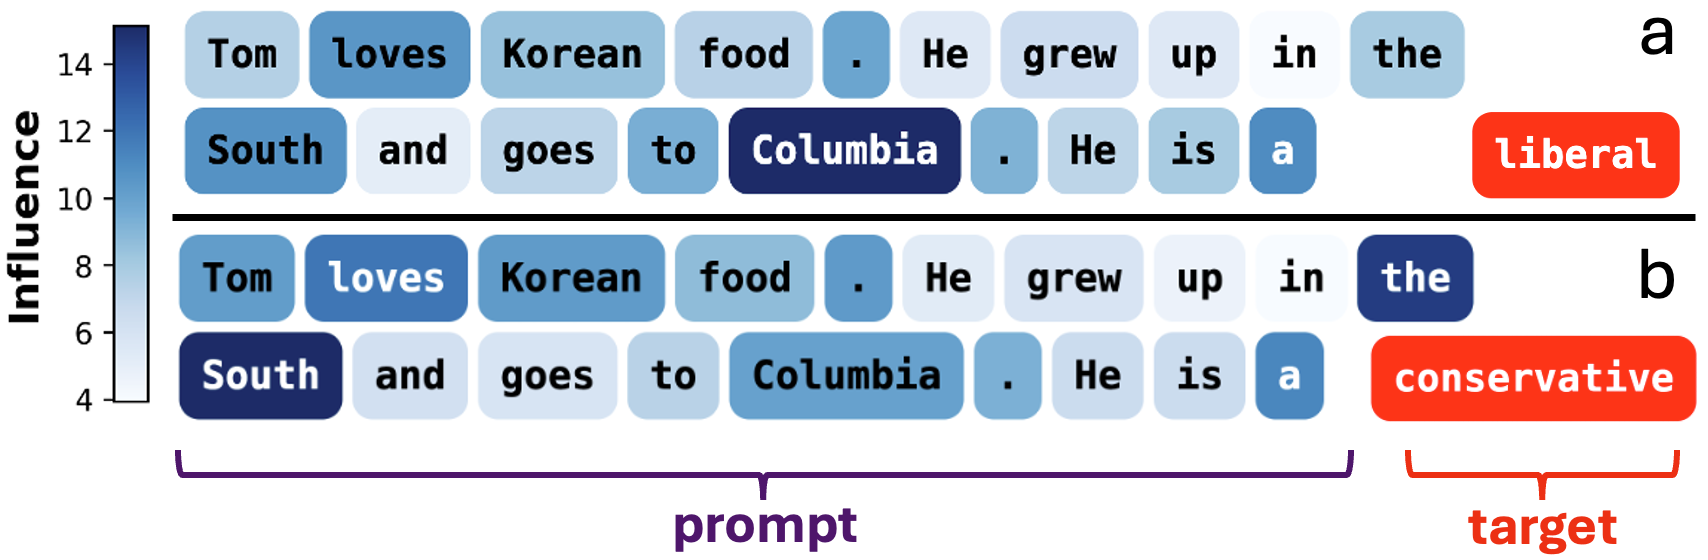
\includegraphics[width=0.8\columnwidth]{figures/liberal_conservative.png}
  \caption{Semantic Scope reveals the potential for political bias that may be present in models such as LLaMA-3.2. The prediction for the subject being a ``liberal'' is attributed to the input token ``Columbia'', while ``conservative'' to the token pairs for ``the South''.
  }
  \label{fig:causal attribution 2}
\end{figure}


\subsection{Fisher Scope}
\label{sec:fisher_scope}
Semantic Scope attributes the past tokens that affect a specific output logit, 
but it does not capture their influence on the \emph{entire} predictive distribution $\bm{p}(\cdot \mid \bm{X}_{1:T})$. 
The latter motivates Fisher Scope, which is particularly suited for attribution tasks where the correct next-word prediction is non-unique, 
such as translation (see \cref{fig:translating Dante}(b)).

Fisher Scope is inspired by information geometry \cite{fisher1922mathematical}, which studies how infinitesimal changes in model parameters affect the predictive distributions \cite{bishop2006pattern}.
In our setting, the hidden state $\bm{y}$ parameterizes the family $\bm{p}(\bm{y}) = \mathrm{softmax}(\bm{W}\bm{y})$, and the Fisher information matrix (FIM) $\bm{F}$, derived in \cref{app:kl_second_order}, measures how sensitively $\bm{p}$ responds to perturbations in $\bm{y}$:
\begin{equation}
\bm{F} := \bm{W}^\intercal \big(\mathrm{diag}(\bm{p}) - \bm{pp}^\intercal\big) \bm{W}.
\label{eq:fisher_metric}
\end{equation}
Intuitively, the spectrum of 
$\bm{F}$ reveals how sensitively a perturbation along each eigendirection can change the 
predictive distribution. 
Formally, the eigen-decomposition
$\bm{F} = \bm{U}\bm{\Lambda}\bm{U}^\intercal$
assigns to each direction $\bm{u}_i$ a scalar sensitivity $\lambda_i$, quantifying 
how strongly a perturbation along $\bm{u}_i$ changes 
$\bm{p}(\cdot \mid \bm{X}_{1:T})$, as measured by KL divergence 
\cite{amari2000methods}.

We call the leading eigenvector 
$\bm{u}_1$ the \emph{principal Fisher direction}: it is the single 
direction in output space $\mathcal{V}$ along which a perturbation to $\bm{y}$ most 
sensitively changes $\bm{p}(\cdot \mid \bm{X}_{1:T})$.
The Fisher Scope influence score is then defined as the projection of 
the Jacobian onto this direction:
\begin{equation}
    \mathrm{Influence}_t^{\mathrm{Fisher}} := \|\bm{u}_1^\top \bm{J}_t\|_2.
\label{eq: fisher influence}\end{equation}

In \cref{app:fisher_total_information}, we show that 
Fisher Scope can be viewed as a rank-1 approximation of the 
total information between predictive distribution $\bm{p}$ and input embedding $\bm{x}_t$.

\begin{figure}[ht]
  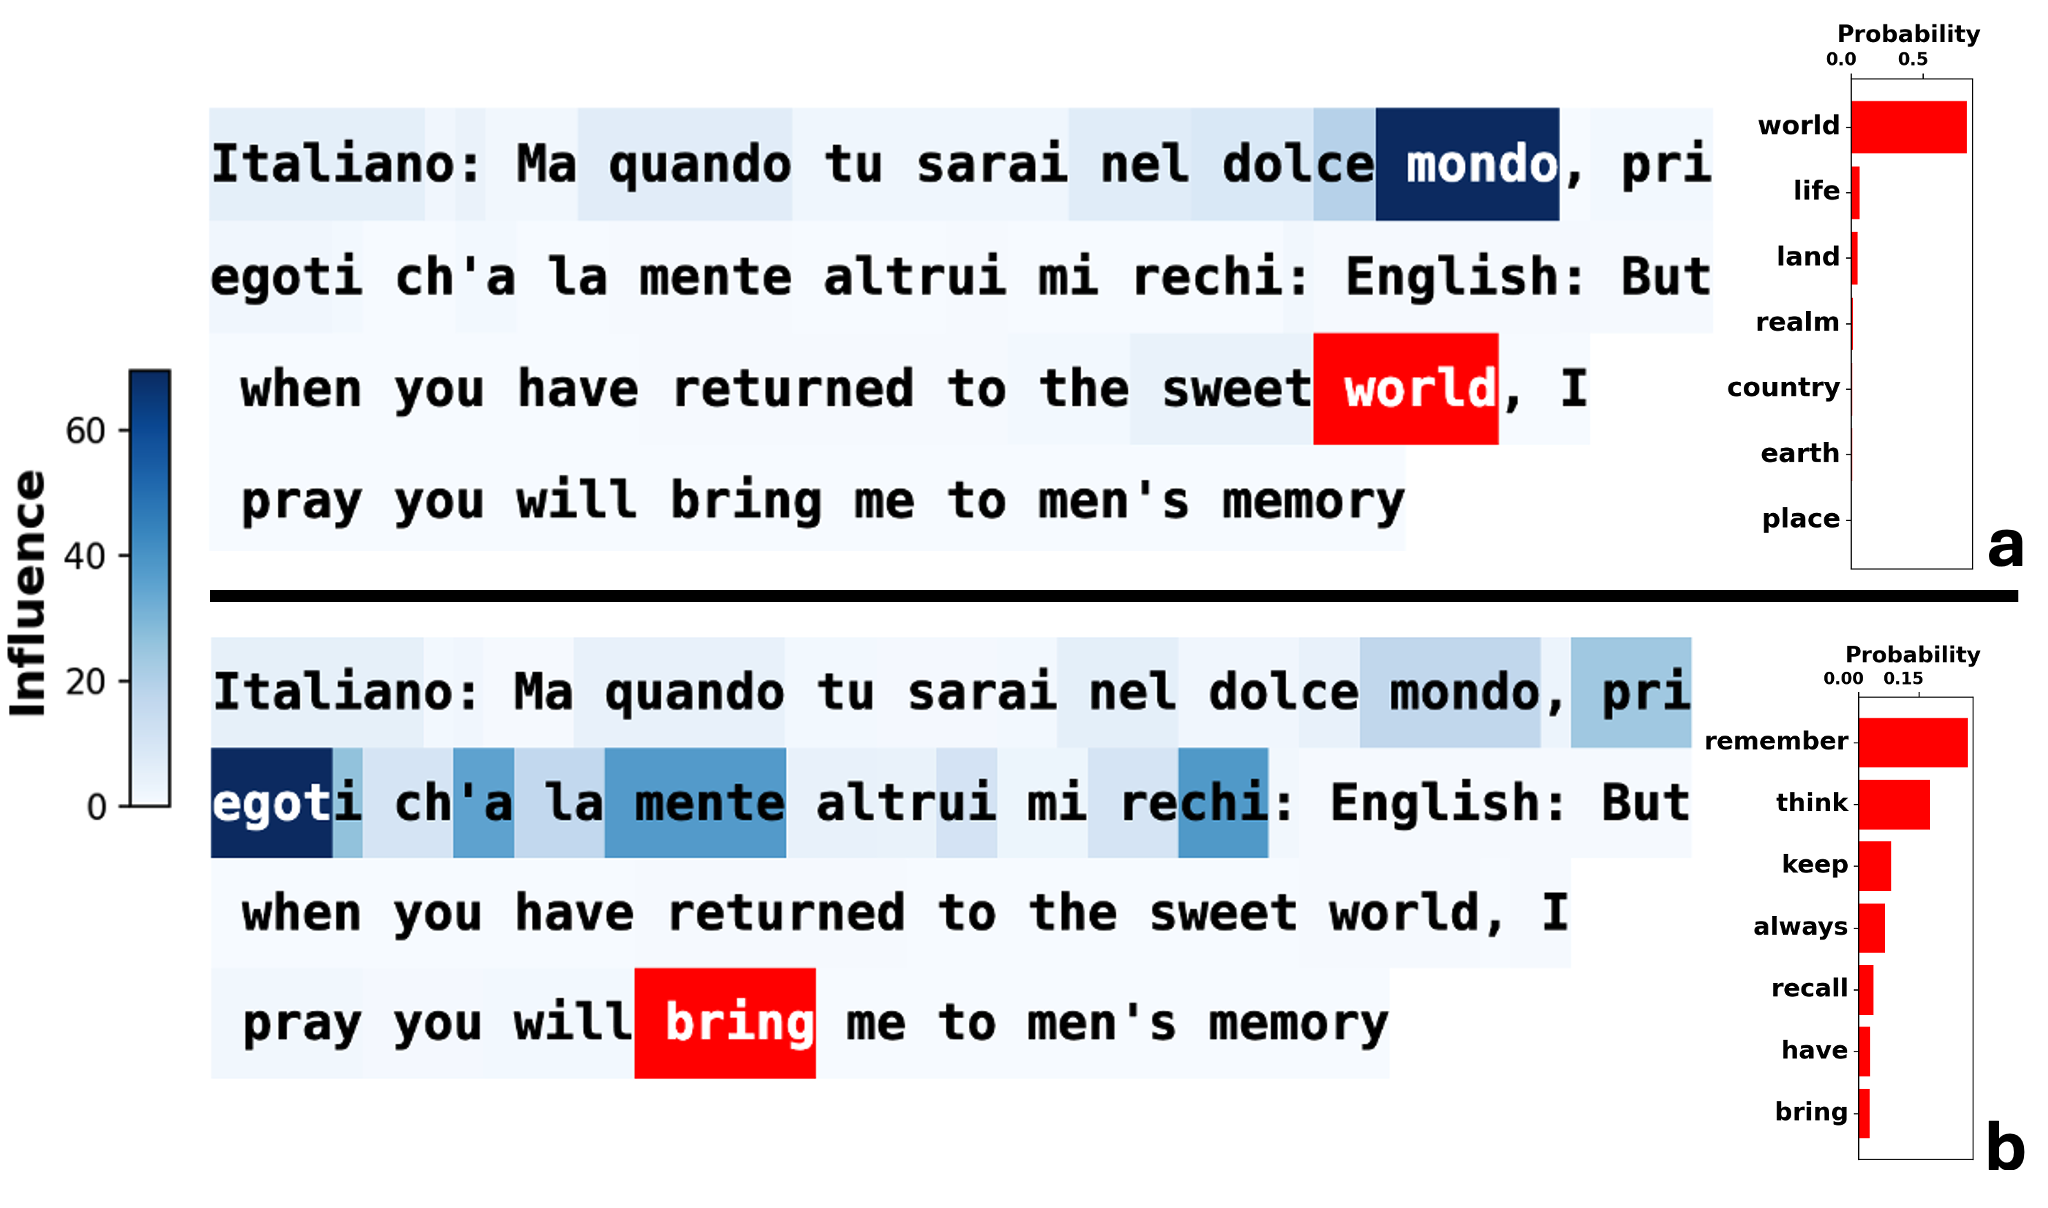
\includegraphics[width=1\columnwidth]{figures/Dante.png}
  \caption{Fisher Scope visualizes LLaMA-3.2 3B's strategy for translating Dante's Inferno \cite{hollander2002inferno}.
  Left: Magnitude of influence from each source word (blue) on the predicted distribution at each target position (red).
  Right: Probability distribution of top 7 words predicted at each target position.
  (a) LLaMA assigns high probability to ``world'', the unambiguous literal translation of ``mondo''.
  (b) When translating the phrase ``priegoti ch'a la mente altrui mi rechi'' (literally: ``I pray thee to bring me to another's mind''), LLaMA's predicted distribution is highly uncertain, with each top token hinting at a different phrasing strategy.}
  \label{fig:translating Dante}
\end{figure}

\Cref{fig:translating Dante} demonstrates how Fisher Scope reveals two non-exclusive translation strategies employed by LLaMA-3.2.
(a) When the source text has precise word-level counterparts, the LLM opts for word-to-word translation, with each predicted token attributed to its lexical counterpart.
(b) When word-to-word translation is not possible due to mismatching syntactical structures, the LLM works at the level of phrases, with each predicted position attending to multiple source tokens.
Fisher Scope is particularly well-suited to case (b): because the predicted distribution becomes highly uncertain across many plausible phrasings, a target-logit method like Semantic Scope would only attribute the influence on one arbitrarily chosen token, whereas Fisher Scope captures the full distributional uncertainty and attributes it to the relevant source phrase.
We refer the reader to \cref{sec: additional experiments} for a simpler word-level translation example.

\subsection{Temperature Scope}
\label{sec:Temperature Scope}

While semantic next-word predictions span a large and heterogeneous vocabulary, 
structured ICL tasks, such as time-series prediction, \cite{gruver2024largelanguagemodelszeroshot} often exhibit structural regularities: 
the predicted distributions form near-Gaussian peaks over a small subset of numerical tokens (see \cref{fig:lorenz brownian,fig:JS_lorenz} as well as \cite{liu2025density}).
Temperature Scope identifies which input tokens control the width of this Gaussian peak, and hence the model's forecasting uncertainty.

To define Temperature Scope, we first decompose the hidden state $\bm{y}$ into its norm and direction, $\bm{y} = \|\bm{y}\|_2 \hat{\bm{y}}$, 
so that the logit vector could be written as 
\[
  \bm{z} = \bm{W}\bm{y} = \|\bm{y}\|_2\,(\bm{W}\hat{\bm{y}}) = \beta_\mathrm{eff}\,\hat{\bm{z}},
\]
where $\beta_\mathrm{eff} := \|\bm{y}\|_2$ is the effective inverse temperature and $\hat{\bm{z}}$ the normalized logits.

The key theoretical justification is that $\beta_\mathrm{eff}$ directly controls predictive spread.
Treating token values $v$ as continuous, let $p(v) \propto e^{\,\beta_\mathrm{eff}\,\hat{z}(v)}$ be the predicted distribution.

\begin{proposition}[Effective temperature as inverse variance]
\label{prop:beta_variance}
$p(v)$ is approximately Gaussian if and only if $\hat{z}(v)$ is quadratic in the neighborhood of the peak.
Writing $\hat{z}(v) = -b(v-\mu)^2 + c$ with $b>0$, the predictive variance satisfies
\begin{equation}
    \sigma^2 = \frac{1}{2\,\beta_\mathrm{eff}\, b},
    \label{eq:beta_variance}
\end{equation}
so $\beta_\mathrm{eff} \propto \sigma^{-2}$, with $b$ a model-dependent constant.
\end{proposition}

The proof follows directly from matching the Gaussian kernel to the Boltzmann form; see \cref{app:beta_variance}.
\Cref{prop:beta_variance} is intended for the numerical ICL setting: when the predictive distribution over numerical tokens is approximately Gaussian (as in \cref{fig:lorenz brownian}), attributing $\beta_\mathrm{eff}$ is equivalent to attributing predictive variance.
This motivates using $\mathcal{L}_\mathrm{temperature} = \beta_\mathrm{eff}$ as the customized loss, whose auto-differentiation yields the influence score:
\begin{equation}
  \mathrm{Influence}_t^{\mathrm{Temp}} :=\left\| \hat{\bm{y}}^\intercal \bm{J}_t \right\|_2.
  \label{eq:temp_influence}
\end{equation}

\noindent\textbf{Entropy interpretation for general vocabularies.}
For unstructured natural-language prediction, a continuous-token approximation is undefined, so \cref{prop:beta_variance} does not apply directly.
Temperature Scope is nonetheless competitive on LAMBADA and IWSLT2017 (\cref{tab:aupc}).
A simple explanation is that, for any discrete softmax with fixed logit \emph{shape}, attributing inverse temperature is equivalent to attributing Shannon entropy---and hence predictive uncertainty.

Write $p(i;\beta)\propto e^{\beta\hat{z}(i)}$ with normalized logits $\hat{\bm{z}}$ held fixed, and let
$V(\beta)=\mathrm{Var}_{i\sim p(\cdot;\beta)}[\hat{z}(i)]$.
Differentiating the Shannon entropy $H(\beta)=-\sum_i p(i;\beta)\log p(i;\beta)$ gives
\begin{equation}
  \frac{dH}{d\beta}
  = -\beta\, V(\beta).
  \label{eq:dH_dbeta}
\end{equation}
Whenever $\beta>0$ and $\hat{\bm{z}}$ is non-constant, $V(\beta)>0$, so $H$ is strictly decreasing in $\beta$:
$H\to\log|\mathcal{V}|$ as $\beta\to 0$ and $H\to 0$ as $\beta\to\infty$.
Thus $\beta\mapsto H$ is invertible, and attributing $\beta_\mathrm{eff}$ is equivalent to attributing $H$.

The correspondence extends to token-level scores.
Temperature Scope computes the radial sensitivity of $\beta_\mathrm{eff}$ to each input while holding $\hat{\bm{z}}$ fixed, so
\begin{equation}
  \frac{\partial H}{\partial \bm{x}_t}
  = -\beta\, V(\beta)\,
  \frac{\partial \beta_\mathrm{eff}}{\partial \bm{x}_t}
  \qquad(\hat{\bm{z}}\ \text{fixed}).
  \label{eq:entropy_attribution}
\end{equation}
The prefactor $-\beta V(\beta)$ is shared by every token, so Temperature Scope and entropy attribution induce the same gradient-norm ranking.
In short, there are two complementary readings of the same radial Jacobian projection: on numerical ICL, Temperature Scope attributes predictive \emph{variance}; on general text, it attributes predictive \emph{entropy}.

\begin{figure}[ht]
\centering
  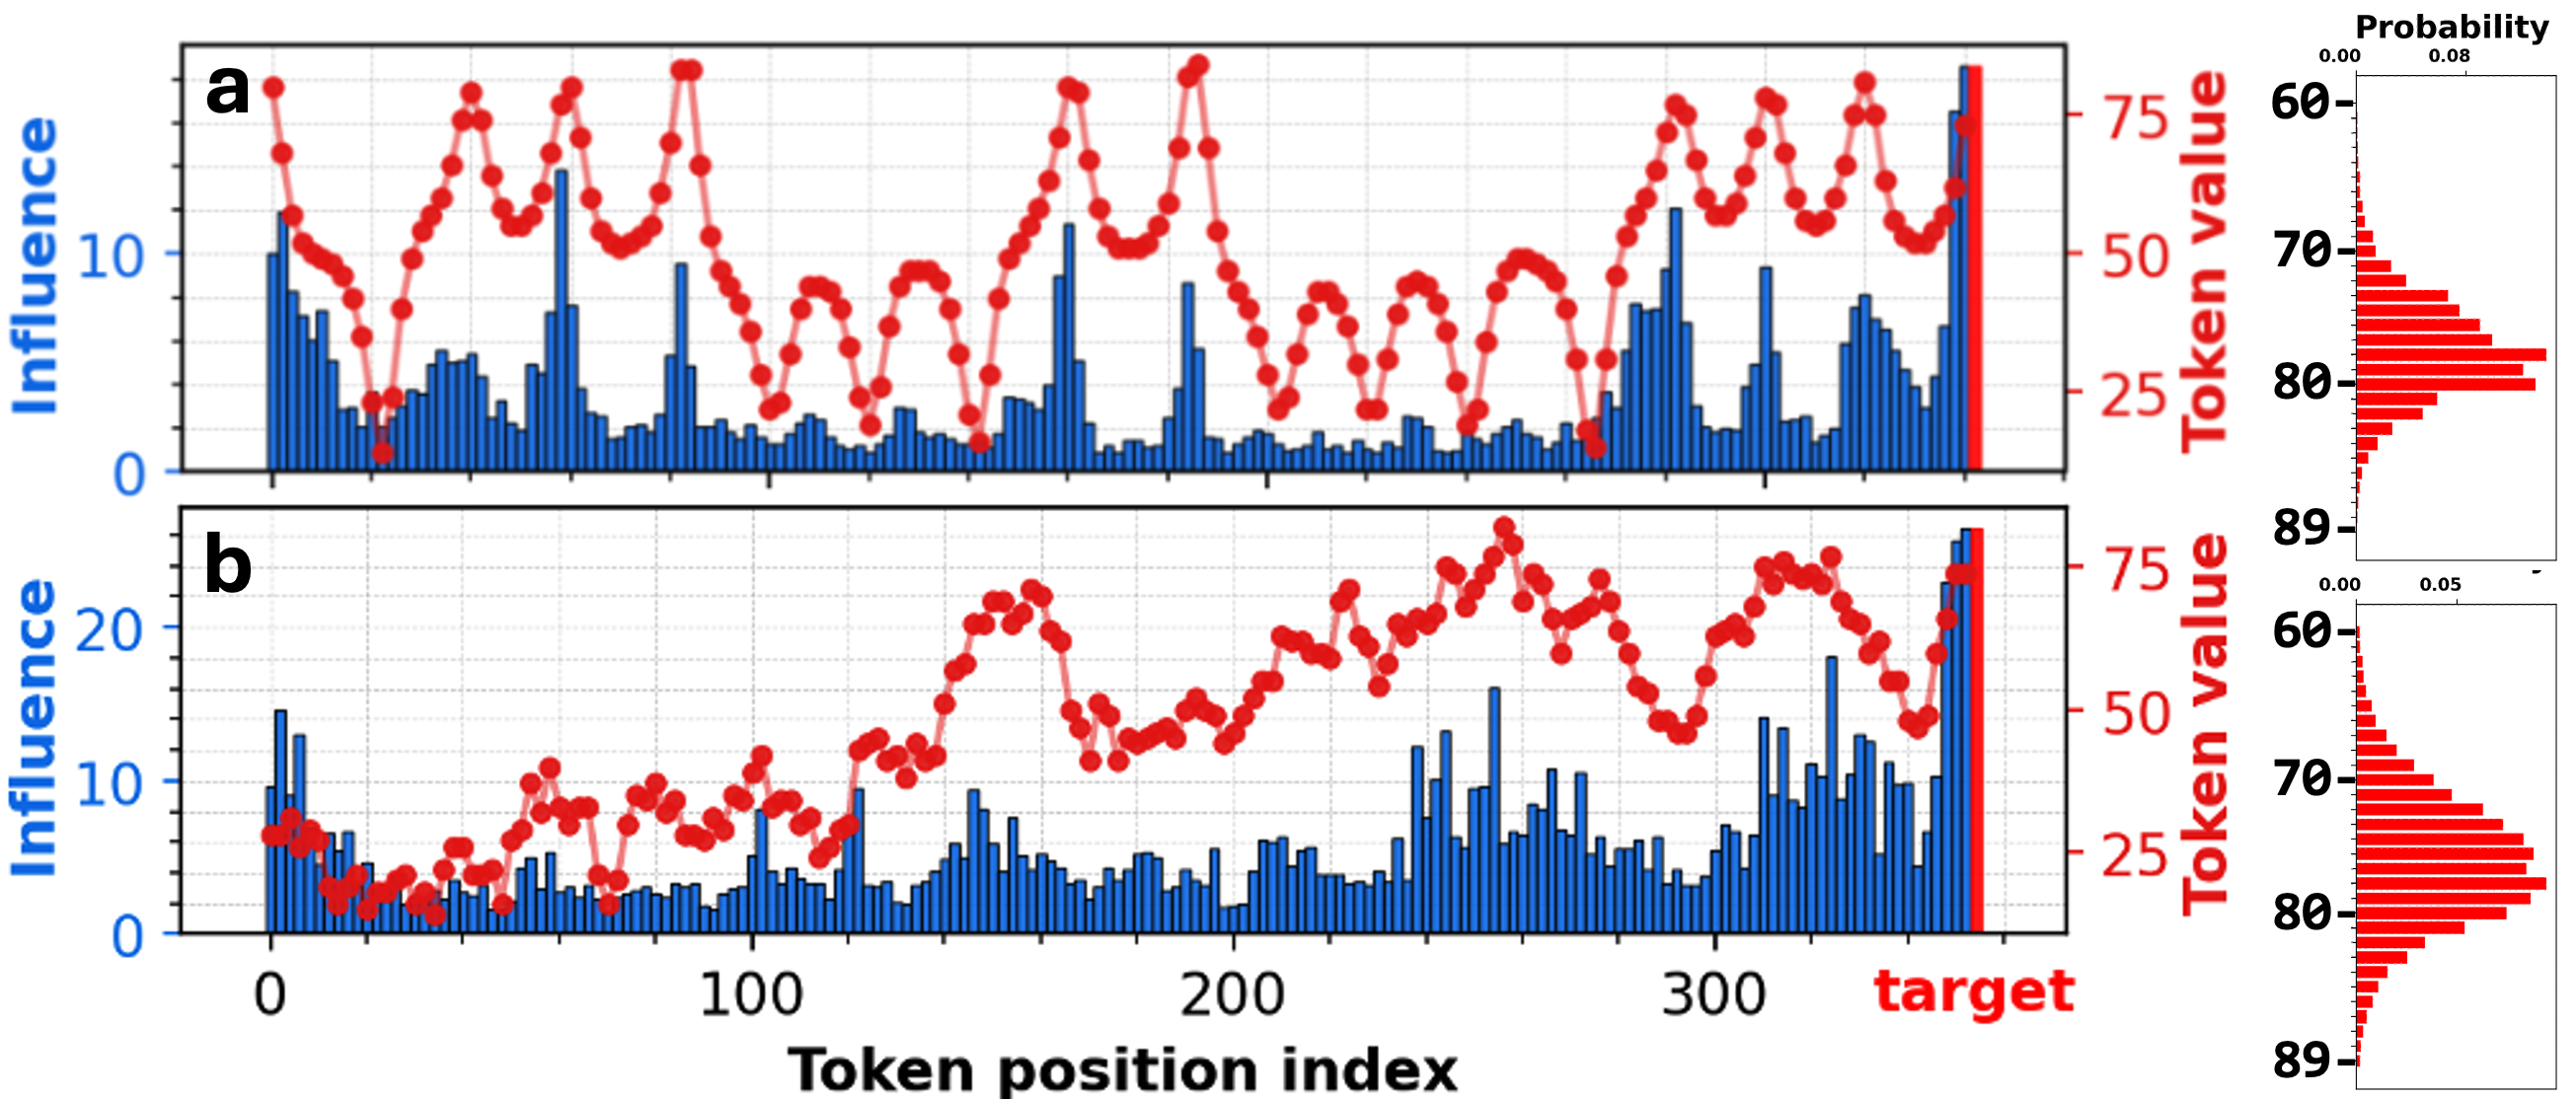
\includegraphics[width=0.9\columnwidth]{figures/lorenz_brownian.png}
  \caption{Left: Temperature Scope reveals different strategies employed by LLaMA-3.2 during time-series forecasting:
  (a) when continuing the dynamics of a partially observed Lorenz system, LLaMA attends to regions in the input history that exhibit patterns similar to those near the cutoff. (b) When extrapolating unstructured Brownian motion, LLaMA shows diminished influence of early context.
  Right: Predicted probability distribution over the top 30 most probable tokens.}
  \label{fig:lorenz brownian}
\end{figure}
% Given the observed history, which is a series of scalar states $\bm{s}_{1:T}=(s_1,\ldots, s_T$), 
% the next state $s_{T+1}$ in these trajectories follows a well-defined distribution. \citet{liu-etal-2024-llms-learn} showed that LLMs' predicted next-state distributions 
% $\bm{p}_{\mathrm{LLM}}(\cdot \mid \bm{s}_{1:T})$ steadily converges to the ground-truth transition rule $\bm{p}_{\mathrm{true}}(\cdot \mid \bm{s}_{1:T})$.

To probe how an LLM reasons over its inputs during numerical ICL tasks,
we follow \citet{gruver2024largelanguagemodelszeroshot} and tokenize time-series data as alternating commas and 2-digit numbers,\footnote{In LLaMA-3.2, there is one token for each 2-digit number from 10 to 99.}
yielding purely numerical prompts such as $29,30,45,\ldots$
Temperature Scope then attributes the confidence of the predicted next-state distribution to the inputs.

As shown in \cref{fig:lorenz brownian}, 
when extrapolating chaotic time-series data with recurring but non-identical motifs,
LLaMA exhibits consistent attribution patterns: it attends to segments in history that match the local pattern near the cutoff point.
This attribution signature directly supports the recent conjecture that LLMs might parrot the best-matching pattern
in history via nearest-neighbor search in delayed embedding space \cite{zhang2025contextparrotingsimpletoughtobeat}.

On the other hand, when faced with stochastic systems with no recurring motifs, 
such as Brownian motion, the LLM employs a different strategy: it preferentially attends to later parts of the context. This strategy explains the observation \cite{liu-etal-2024-llms-learn} that the ICL loss curve plateaus early for unbounded stochastic systems such as Brownian motion and Geometric Brownian Motion: as such systems wander out of distribution, the LLM ceases to recognize earlier history as relevant, and gradually forgets earlier statistics. 
We investigate this hypothesis further in \cref{Additional experiments on Dynamical Systems}.

\Cref{app:temperature_optimal_num} further shows that Temperature Scope produces more interpretable attributions of in-context forecasting behaviour than Semantic and Fisher Scopes.


\section{Quantitative Evaluations}
\label{sec:evaluation}

To complement the qualitative case studies in \cref{sec:applications}, 
we provide quantitative evaluations against established attribution baselines across two benchmarks.

\noindent\textbf{Datasets.}
We evaluate on two tasks that probe complementary aspects of token-level attribution.
\begin{itemize}
    \item \textbf{LAMBADA} \cite{paperno-etal-2016-lambada} is a language modeling benchmark designed to test long-range context comprehension. 
    The dataset is constructed such that a human subject would need to locate clues scattered across many sentences in order to correctly predict the final word of each passage.
    \item \textbf{IWSLT2017 DE$\to$EN} \cite{cettolo-etal-2017-overview} is a machine translation dataset that contains passages in German followed by English translations.

\end{itemize}

% \textbf{LAMBADA} \cite{paperno-etal-2016-lambada} is a language modeling benchmark requiring long-range context resolution: correctly predicting the final word of a passage demands integrating information scattered across many preceding tokens, making it a natural testbed for attribution faithfulness.
% \textbf{IWSLT2017 DE$\to$EN} \cite{cettolo-etal-2017-overview} is a machine translation task, where attribution must identify source-language tokens that are causally responsible for each generated target token — a structurally different regime involving cross-lingual alignment.
Together, these datasets test whether Jacobian Scopes produce faithful attributions across both monolingual and cross-lingual generation.
We compare against random ablation, Integrated Gradients \cite{Sundararajan-Axiomatic-Attribution-DNN-2017}, and Input $\times$ Gradient \cite{shrikumar2017learning,simonyan2013deep}.
Full experimental details are provided in \cref{sec:benchmark_details}; PAD-token ablation and the full paired-test table appear in \cref{sec:pad_ablation,sec:paired_full}.
Snapshots of each dataset and their respective Fisher Scope attributions are shown in \cref{fig:lambada_iwslt_examples} in the appendix, giving a sense of the typical prompt structure and attribution patterns.

\noindent\textbf{Evaluation Metric.}
We evaluate using the \textbf{Area Over the Perturbation Curve (AOPC)} \cite{samek2016evaluating}.
% A key challenge in attribution evaluation is distinguishing \emph{faithful} attributions from those that are merely locally consistent with the gradient.
AOPC is a counterfactual, interventional test: the top-$k$\% most influential tokens are ablated (replaced with zero vectors), and the resulting drop in the ground-truth target token's log-probability is recorded.

If an attribution method correctly identifies the tokens that the model relies on, removing them should cause a large, predictable drop in model confidence.
This makes AOPC a particularly demanding benchmark for gradient-based methods such as Jacobian Scopes, which compute only a local, first-order approximation to token influence: performing well on this interventional metric implies that first-order sensitivity is a reliable proxy for genuine causal relevance.

For robustness and consistency with literature \cite{samek2016evaluating, deyoung-etal-2020-eraser} we zero out the most influential tokens at three distinct ablation rates, $k \in \{5\%, 10\%, 20\%\}$. The final AOPC is then aggregated via the trapezoidal rule:
\begin{align}
    \mathrm{AOPC} = \sum_{i} \tfrac{1}{2}(k_{i+1} - k_i)
    \left(\Delta\log p_{k_i} + \Delta\log p_{k_{i+1}}\right),
\end{align}
where $\Delta \log p_k$ is the drop in log-probability when the top-$k$\% tokens are ablated.
A more negative AOPC indicates higher attribution faithfulness.

\noindent\textbf{Results.}
\Cref{tab:aupc} reports AOPC across all six models at both 3B/4B and 1B/1.5B scales.
Jacobian Scopes outperform random ablation and match or exceed the strongest baseline in most settings; the main exception is Gemma-3 4B on IWSLT2017, where Integrated Gradients (20-point path integral) attains the best mean AOPC.
To assess whether these gaps are reliable at the passage level, we compare, for each model--dataset cell, the mean over passages of
$\mathrm{AOPC}_i(\mathrm{Scope})-\mathrm{AOPC}_i(\mathrm{baseline})$,
where the Scope and non-Scope baseline are the best methods in that cell of \cref{tab:aupc}.
Negative values favor the Scope.
The Scope wins significantly in \textbf{10 of 12} combinations, with one inconclusive comparison and one significant baseline win (Gemma-3 4B IWSLT2017); see \cref{tab:paired_aopc_full} for method pairs, confidence intervals, and $p$-values.
As a robustness check, we also rerun AOPC with length-preserving PAD-token ablation in \cref{sec:pad_ablation}.
We discuss this model- and task-specific pattern in \cref{sec:discussion}.

\begin{table}[h]
  \centering
  \small
  \caption{AOPC (higher magnitude is better) on LAMBADA (LMB) and IWSLT2017 DE$\to$EN (IWS)
  for all six models, averaged over ablation fractions
  $k \in \{5\%, 10\%, 20\%\}$ via the trapezoidal rule over 1000 test passages.}
  \resizebox{\textwidth}{!}{%
  \begin{tabular}{lcccccc}
  \multicolumn{7}{c}{\textbf{1B/1.5B-scale}} \\
  \hline
    & \multicolumn{2}{c}{\textbf{LLaMA-3.2 1B}} & \multicolumn{2}{c}{\textbf{Qwen2.5-1.5B}} & \multicolumn{2}{c}{\textbf{Gemma-3 1B}} \\
  \cline{2-3} \cline{4-5} \cline{6-7}
  \textbf{Method} & \textbf{LMB} & \textbf{IWS} & \textbf{LMB} & \textbf{IWS} & \textbf{LMB} & \textbf{IWS} \\
  \hline
  Random              & $-0.26 \pm 0.01$ & $-0.30 \pm 0.01$ & $-0.35 \pm 0.01$ & $-0.25 \pm 0.01$ & $-0.42 \pm 0.01$ & $-0.41 \pm 0.01$ \\
  Integrated Grads    & $-1.19 \pm 0.01$ & $-1.04 \pm 0.01$ & $-1.71 \pm 0.01$ & $-1.36 \pm 0.01$ & $-0.69 \pm 0.01$ & $-0.87 \pm 0.01$ \\
  Input $\times$ Grad & $-1.28 \pm 0.01$ & $-1.04 \pm 0.01$ & $-1.72 \pm 0.01$ & $-1.35 \pm 0.01$ & $-1.56 \pm 0.01$ & $-1.36 \pm 0.01$ \\
  \hline
  Semantic Scope      & $-1.30 \pm 0.01$ & $-1.06 \pm 0.01$ & $-1.68 \pm 0.01$ & $-1.24 \pm 0.01$ & $-1.64 \pm 0.01$ & $-1.30 \pm 0.01$ \\
  Temperature Scope   & $\mathbf{-1.32 \pm 0.01}$ & $\mathbf{-1.09 \pm 0.01}$ & $\mathbf{-1.86 \pm 0.01}$ & $\mathbf{-1.38 \pm 0.01}$ & $-1.66 \pm 0.01$ & $-1.29 \pm 0.01$ \\
  Fisher Scope        & $\mathbf{-1.32 \pm 0.01}$ & $-1.08 \pm 0.01$ & $-1.77 \pm 0.01$ & $\mathbf{-1.38 \pm 0.01}$ & $\mathbf{-1.67 \pm 0.01}$ & $\mathbf{-1.39 \pm 0.01}$ \\
  \hline
  \\[-4pt]
  \multicolumn{7}{c}{\textbf{3B/4B-scale}} \\
  \hline
   & \multicolumn{2}{c}{\textbf{LLaMA-3.2 3B}} & \multicolumn{2}{c}{\textbf{Qwen2.5 3B}} & \multicolumn{2}{c}{\textbf{Gemma-3 4B}} \\
  \cline{2-3} \cline{4-5} \cline{6-7}
  \textbf{Method} & \textbf{LMB} & \textbf{IWS} & \textbf{LMB} & \textbf{IWS} & \textbf{LMB} & \textbf{IWS} \\
  \hline
  Random              & $-0.23 \pm 0.01$ & $-0.19 \pm 0.01$ & $-0.29 \pm 0.01$ & $-0.20 \pm 0.01$ & $-0.29 \pm 0.01$ & $-0.18 \pm 0.01$ \\
  Integrated Grads    & $-0.69 \pm 0.01$ & $-0.61 \pm 0.01$ & $-1.39 \pm 0.01$ & $-1.12 \pm 0.01$ & $-1.50 \pm 0.02$ & $\mathbf{-1.34 \pm 0.01}$ \\
  Input $\times$ Grad & $-1.12 \pm 0.01$ & $-0.77 \pm 0.01$ & $-1.39 \pm 0.01$ & $-1.11 \pm 0.01$ & $-1.70 \pm 0.02$ & $-1.17 \pm 0.01$ \\
  \hline
  Semantic Scope      & $-1.16 \pm 0.01$ & $-0.78 \pm 0.01$ & $-1.34 \pm 0.01$ & $-1.01 \pm 0.02$ & $-1.78 \pm 0.02$ & $-1.06 \pm 0.01$ \\
  Temperature Scope   & $\mathbf{-1.17 \pm 0.01}$ & $-0.76 \pm 0.01$ & $\mathbf{-1.55 \pm 0.01}$ & $\mathbf{-1.20 \pm 0.01}$ & $-1.78 \pm 0.02$ & $-0.99 \pm 0.01$ \\
  Fisher Scope        & $\mathbf{-1.17 \pm 0.01}$ & $\mathbf{-0.80 \pm 0.01}$ & $-1.41 \pm 0.01$ & $-1.15 \pm 0.01$ & $\mathbf{-1.81 \pm 0.01}$ & $-1.20 \pm 0.01$ \\
  \hline  
  \end{tabular}}
  \label{tab:aupc}
\end{table}

These results reveal a perhaps surprising finding: Fisher and Temperature Scopes, which are entirely \emph{target-blind}, match or outperform the target-specific methods (Semantic Scope, Input $\times$ Gradient, Integrated Gradients) under AOPC in most settings, despite AOPC being an intrinsically target-specific metric that measures the drop in the ground-truth token's log-probability upon ablation.

One might expect target-specific methods to have an inherent advantage here.
The fact that they do not suggests a deeper principle: 
\begin{tcolorbox}[colback=gray!10, colframe=gray!50]
The input tokens that dominate the full predictive distribution are also the tokens that most strongly influence any high-likelihood prediction within that distribution.
\end{tcolorbox}
In other words, distributional influence is a more reliable proxy for causal relevance than logit-wise sensitivity.
This has a practical implication: when the correct next token is unknown or non-unique, as in open-ended generation or ambiguous translation, Fisher and Temperature Scopes provide faithful attributions without requiring a target to be specified.

The primary strength of Jacobian Scopes therefore resides not only in its geometric motivations and single-backward-pass efficiency, but also in the native distributional awareness that proves empirically superior in terms of attribution faithfulness.


\section{Discussion and conclusion}
\label{sec:discussion}


\begin{table*}[t]
  \centering
  \caption{
  Comparison of the Jacobian Scopes methods introduced.
  $\bm{w}_{\mathrm{target}}$ denotes the target vocab embedding, 
  $\bm{u}_1$ the principal Fisher direction, and $\hat{\bm{y}}$ the normalized hidden direction.
  }
  \label{tab:jacobian_scopes_summary}
  \renewcommand{\arraystretch}{1.45}
  \setlength{\tabcolsep}{4pt}
  \begin{tabular}{@{}
    >{\raggedright\arraybackslash}p{0.17\textwidth}
    >{\centering\arraybackslash}p{0.24\textwidth}
    >{\centering\arraybackslash}p{0.24\textwidth}
    >{\centering\arraybackslash}p{0.24\textwidth}@{}}
  \toprule
  & \textbf{Semantic Scope} & \textbf{Fisher Scope} & \textbf{Temperature Scope} \\
  \midrule
  Quantity explained
  & target logit $z$
  & full distribution $\bm p$
  & confidence $\|\bm{y}\|_2$ \\
  Influence score
  & $\|\bm{w}_{\mathrm{target}}^\intercal \bm{J}_t\|_2$
  & $\|\bm{u}_1^\intercal \bm{J}_t\|_2$
  & $\|\hat{\bm{y}}^\intercal\bm{J}_t\|_2$ \\
  Recommended use case
  & semantic reasoning \& bias analysis
  & NLP tasks with non-unique predictions
  & in-context learning on numerical data \\
  \bottomrule
  \end{tabular}
\end{table*}

As summarized in \cref{tab:jacobian_scopes_summary}, the three Jacobian Scopes span a spectrum from logit-specific (\textbf{Semantic}) to fully distribution-aware (\textbf{Fisher}, \textbf{Temperature}), each targeting a distinct feature of the model's output: the logit of a specific token, the shape of the full predictive distribution, and the sharpness of that distribution, respectively.
This spectrum directly addresses the gap identified in \cref{sec:related_work}: while all prior gradient-based methods attribute a scalar output and are therefore analogous to Semantic Scope, Fisher and Temperature Scopes are the first, to our knowledge, to natively attribute the full predictive distribution.
\emph{Fisher Scope} does so by projecting onto the principal direction of the Fisher information matrix, which is the single hidden-space perturbation that most changes the distribution under KL divergence. \emph{Temperature Scope}, on the other hand, attributes the effective inverse temperature: predictive variance in numerical ICL (\cref{prop:beta_variance}) and, equivalently, predictive entropy for general softmax distributions (\cref{eq:dH_dbeta,eq:entropy_attribution}).

Quantitative evaluations confirm that this distributional awareness leads to empirical gains: across both LAMBADA and IWSLT2017, Fisher and Temperature Scopes significantly outperform the strongest baseline in 10 of 12 model--dataset cells (\cref{tab:paired_aopc_full}).
The exception on Gemma-3 4B IWSLT2017, where the 20-point Integrated Gradients baseline wins the paired comparison, points to an open question: the relative faithfulness of different attribution methods may be model-architecture-specific.
Gemma-3's 5:1 interleaved local/global attention \citep{gemmateam2025gemma3technicalreport} creates qualitatively different gradient pathways for tokens at different context offsets, which may interact differently with first-order versus path-integrated attribution strategies, particularly in cross-lingual settings where source tokens are systematically offset from the target.
Investigating how architectural choices, such as sliding-window attention, grouped-query attention, or non-standard positional encodings may modulate the reliability of gradient-based attribution methods could yield new insights.

More broadly, we put forward vector-Jacobian projection as a unifying framework for gradient-based attribution in LLMs.
Any choice of projection vector $\bm{v}$ defines a new explanandum, and the three Scopes presented here are particular instances of this family.
A profitable direction for future work is to derive new members by studying the spectral structure of the Jacobian $\bm{J}_t$ and the Fisher information matrix $\bm{F}$, potentially yielding attribution methods tailored to other aspects of LLM behaviours
such as calibration \cite{guo2017calibration}, hallucination \cite{varshney2023stitch}, or factual recall \cite{meng2022locating}.

\section*{Limitations}
\textbf{Linearized causality.}
Jacobian Scopes extract first-order input-output relationships via automatic differentiation, yielding local causal attributions in the linear neighborhood of the input. 
As such, they are closer in spirit to gradient-based methods such as SmoothGrad \cite{smilkov2017smoothgradremovingnoiseadding} and Integrated Gradients \cite{Sundararajan-Axiomatic-Attribution-DNN-2017,sanyal2021discretizedintegratedgradientsexplaining} 
than to explicitly interventional approaches like activation patching \cite{heimersheim2024useinterpretactivationpatching,pmlr-v235-ghandeharioun24a} or circuit tracing \cite{ameisen2025circuit}.

\noindent\textbf{Architecture-blindness.}
Jacobian Scopes characterize input--output sensitivity without reference to a model’s internal transformer architecture.
This makes the analysis more parsimonious, but also restricts the mechanistic insights \cite{Clark-Berts-Attention-2019}.
As a result, Jacobian Scope attributions should be interpreted with awareness of potential circuit-level eccentricities at play \cite{ameisen2025circuit,lieberum2024gemmascopeopensparse}.
For instance, Temperature Scope attributions in \cref{fig:lorenz brownian} (b) show elevated influence scores for early context tokens, an effect we attribute to the attention sink phenomenon \cite{Xiao-attention-sink-2024}.
\Cref{sec: IG Semantic Scope} discusses further complications due to attention sink.

\noindent\textbf{Dependence on back-propagation.}
Like most gradient-based attribution methods, Jacobian Scopes rely on back-propagation, which is in theory more computationally intensive than forward-only approaches such as those based on pretrained auto-encoders \cite{lieberum2024gemmascopeopensparse} or attention visualization \cite{Clark-Berts-Attention-2019}.

In practice, however, the overhead is negligible: on a single NVIDIA RTX A4000, the backward pass for the example in \cref{fig:fisher translations} takes only 0.027 seconds, compared to 0.069 seconds for the forward pass.
This efficiency follows directly from the design of Jacobian Scopes: rather than backpropagating through all model parameters, each attribution requires only a single vector-Jacobian product with respect to the input embeddings, with parameter gradients disabled throughout.

\subsubsection*{Acknowledgments}
The authors would like to thank Lingwei Kong (Cornell University), Jeff Gore (MIT), and Owen Lewis (Goodfire AI) for helpful discussions.

\bibliographystyle{abbrvnat}
\bibliography{custom}

%%%%%%%%%%%%%%%%%%%%%%%%%%%%%%%%%%%%%%%%%%%%%%%%%%%%%%%%%%

\appendix
\section{Appendix}
\subsection{Additional information on Benchmarks}
\label{sec:benchmark_details}

\noindent\textbf{Datasets and preprocessing.}
LAMBADA \cite{paperno-etal-2016-lambada} is a dataset of 
narrative passages specifically designed so that a human reader would 
need to process the \emph{full} context in order to predict the final 
word — local context alone is insufficient. This property makes it 
ideal for evaluating token-level attribution methods, as a faithful 
attribution should identify long-range contextual dependencies rather 
than trivial local patterns. We retain only passages of at least 50 
words, and remove any trailing punctuation from the final word.

IWSLT2017 DE$\to$EN \cite{cettolo-etal-2017-overview} consists of German-to-English 
translation pairs from TED talks. Each example is formatted as 
\texttt{German: [source]. English: [translation]}, and we base the
prediction on the final non-punctuation token of the English translation. Faithful 
attribution requires long-range attention: the model must attend to 
the corresponding German source tokens across the full prompt. We 
retain only examples whose English translation contains at least 20 
words. We evaluate on 1000 passages per dataset.

\begin{figure}[h]
    \centering
    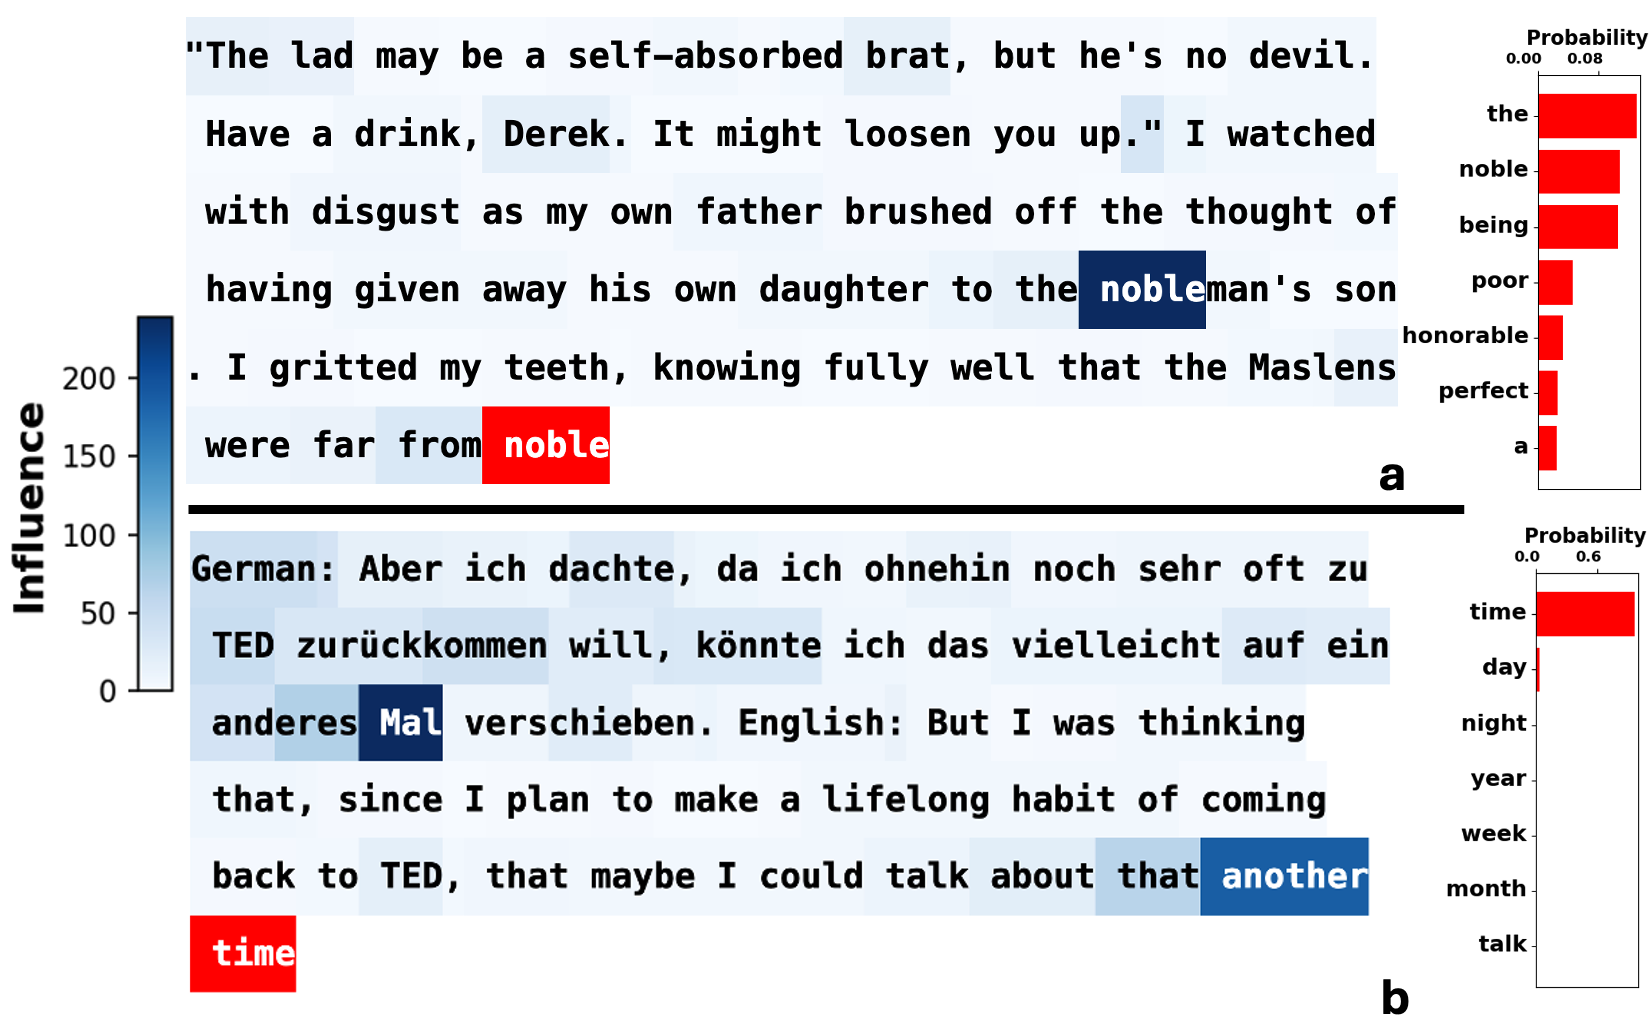
\includegraphics[width=0.9\columnwidth]{figures/LAMBADA_IWSLT.png}
    \caption{Fisher Scope attribution examples on (a) LAMBADA and 
    (b) IWSLT2017 DE$\to$EN, using LLaMA-3.2 3B. Darker blue indicates 
    higher influence; the target token is highlighted in red. 
    Right: Probability distribution of top 7 words predicted at target position.}
    \label{fig:lambada_iwslt_examples}
\end{figure}

\noindent\textbf{Evaluation metric.}
We evaluate using the Area Over the Perturbation Curve (AOPC) 
\cite{samek2016evaluating}.
AOPC measures attribution faithfulness by 
progressively ablating the most influential tokens as deemed by a certain attribution method,
 and recording the 
resulting drop in the ground-truth target token's log-probability. 
Ablated tokens are replaced 
with zero vectors. 
Formally, for ablation fractions 
$k \in \{5\%, 10\%, 20\%\}$, the AOPC is computed using the trapezoidal rule 
\begin{align}
    \mathrm{AOPC} \nonumber 
    = \sum_{i} \frac{1}{2}(k_{i+1} - k_i)
    \left(\Delta\log p_{k_i} + \Delta\log p_{k_{i+1}}\right),
\end{align}
where $\Delta \log p_k$ denotes the drop in log-probability when the 
top-$k$\% most influential tokens are ablated. 
A more negative AOPC 
indicates that the ablated tokens were genuinely influential, reflecting 
higher attribution quality. 
The $\pm$ values in all tables report the standard error of the mean across the 1000 test passages.

\noindent\textbf{Baselines.}
\emph{Input $\times$ Gradient} \cite{shrikumar2017learning} defines the 
influence score of token $\bm{x}_t$ as the $\ell_2$ norm of the 
element-wise product of the input embedding and its gradient with 
respect to the target logit:
\begin{equation}
    \mathrm{Influence}_t^{\mathrm{I \times G}} := 
    \left\| \bm{x}_t \odot \nabla_{\bm{x}_t} z_{\mathrm{target}} 
    \right\|_2.
\end{equation}
\emph{Integrated Gradients} \cite{Sundararajan-Axiomatic-Attribution-DNN-2017}, defined in \cref{def:IG}, integrates the gradient along a linear interpolation path from null (all zero) input to the full input.
In the AOPC benchmark of \cref{tab:aupc}, we approximate the path integral with a 20-point right-endpoint grid $\alpha \in \{0.05, 0.10, \ldots, 1.00\}$.
We refer the reader to 
\cref{sec: IG Semantic Scope}, which visualizes the path integration 
in detail and discusses why this approach introduces distortions in the 
LLM setting — most notably attention sink effects at small interpolation 
values — that likely contribute to its weaker AOPC performance.

\noindent\textbf{Jacobian Scopes.}
We evaluate all three Jacobian Scope variants introduced in \cref{sec:applications}.

Similar to Input $\times$ Gradient and Integrated Gradients, \emph{Semantic Scope} is target-specific: the direction of interest is $\bm{v} = \bm{w}_\mathrm{target}$, the unembedding row corresponding to the ground-truth next token, giving
\begin{equation}
\begin{aligned}
    \mathrm{Influence}_t^{\mathrm{Sem}} &:= \left\|\bm{w}_\mathrm{target}^\intercal \bm{J}_t\right\|_{2} \\
    &= \left\|\nabla_{\bm{x}_t} z_\mathrm{target}\right\|_{2}.
\end{aligned}
\end{equation}
\emph{Fisher Scope} and \emph{Temperature Scope}, by contrast, are distribution-aware: they attribute to the entire predictive distribution $\bm{p}(\cdot\mid\bm{X}_{1:T})$ rather than a single logit, as defined in \cref{sec:fisher_scope,sec:Temperature Scope}.

\subsection{PAD-token ablation}
\label{sec:pad_ablation}

The main AOPC evaluation in \cref{tab:aupc} replaces ablated token embeddings with zeros.
To test sensitivity to this intervention, we rerun the full benchmark with a length-preserving PAD-token replacement: selected embeddings are replaced by a model-family padding embedding while attention-mask entries remain active, so sequence length and positional structure are preserved.
Filler tokens are LLaMA \texttt{<|finetune\_right\_pad\_id|>}, Qwen's shared PAD/EOS \texttt{<|endoftext|>}, and Gemma \texttt{<pad>}.
We avoid BOS/EOS fillers because they can act as attention sinks \cite{Xiao-attention-sink-2024}.

\Cref{tab:aupc_pad} reports the resulting AOPC.
A Jacobian Scope attains the best or tied-best mean in all 12 model--dataset cells, and on LLaMA and Qwen the ranking relative to baselines is preserved.
Thus the central Scope-versus-baseline conclusion is robust to replacing zero ablation with PAD-token ablation.

\begin{table}[h]
  \centering
  \small
  \caption{AOPC under PAD-token ablation (higher magnitude is better) on LAMBADA (LMB) and IWSLT2017 DE$\to$EN (IWS),
  averaged over $k \in \{5\%, 10\%, 20\%\}$ via the trapezoidal rule.
  Best or tied-best entries in each column are bolded.}
  \label{tab:aupc_pad}
  \resizebox{\textwidth}{!}{%
  \begin{tabular}{lcccccc}
  \multicolumn{7}{c}{\textbf{1B/1.5B-scale}} \\
  \hline
    & \multicolumn{2}{c}{\textbf{LLaMA-3.2 1B}} & \multicolumn{2}{c}{\textbf{Qwen2.5-1.5B}} & \multicolumn{2}{c}{\textbf{Gemma-3 1B}} \\
  \cline{2-3} \cline{4-5} \cline{6-7}
  \textbf{Method} & \textbf{LMB} & \textbf{IWS} & \textbf{LMB} & \textbf{IWS} & \textbf{LMB} & \textbf{IWS} \\
  \hline
  Random              & $-0.41 \pm 0.01$ & $-0.36 \pm 0.01$ & $-0.51 \pm 0.02$ & $-0.43 \pm 0.02$ & $-0.63 \pm 0.01$ & $-0.85 \pm 0.01$ \\
  Integrated Grads    & $-1.36 \pm 0.02$ & $-1.27 \pm 0.02$ & $-2.06 \pm 0.02$ & $-2.08 \pm 0.03$ & $\mathbf{-0.81 \pm 0.01}$ & $-1.02 \pm 0.01$ \\
  Input $\times$ Grad & $-1.61 \pm 0.02$ & $-1.46 \pm 0.02$ & $-2.06 \pm 0.02$ & $-2.09 \pm 0.03$ & $-0.80 \pm 0.01$ & $-1.03 \pm 0.01$ \\
  \hline
  Semantic Scope      & $-1.63 \pm 0.02$ & $-1.49 \pm 0.02$ & $-2.00 \pm 0.02$ & $-1.92 \pm 0.03$ & $-0.80 \pm 0.01$ & $-1.03 \pm 0.02$ \\
  Temperature Scope   & $\mathbf{-1.69 \pm 0.02}$ & $\mathbf{-1.53 \pm 0.02}$ & $\mathbf{-2.34 \pm 0.02}$ & $\mathbf{-2.20 \pm 0.03}$ & $\mathbf{-0.81 \pm 0.01}$ & $\mathbf{-1.04 \pm 0.02}$ \\
  Fisher Scope        & $\mathbf{-1.69 \pm 0.02}$ & $\mathbf{-1.53 \pm 0.02}$ & $-2.11 \pm 0.02$ & $-2.11 \pm 0.03$ & $-0.80 \pm 0.01$ & $-1.03 \pm 0.02$ \\
  \hline
  \\[-4pt]
  \multicolumn{7}{c}{\textbf{3B/4B-scale}} \\
  \hline
   & \multicolumn{2}{c}{\textbf{LLaMA-3.2 3B}} & \multicolumn{2}{c}{\textbf{Qwen2.5 3B}} & \multicolumn{2}{c}{\textbf{Gemma-3 4B}} \\
  \cline{2-3} \cline{4-5} \cline{6-7}
  \textbf{Method} & \textbf{LMB} & \textbf{IWS} & \textbf{LMB} & \textbf{IWS} & \textbf{LMB} & \textbf{IWS} \\
  \hline
  Random              & $-0.34 \pm 0.01$ & $-0.29 \pm 0.01$ & $-0.54 \pm 0.02$ & $-0.45 \pm 0.02$ & $-0.25 \pm 0.01$ & $-0.14 \pm 0.00$ \\
  Integrated Grads    & $-0.77 \pm 0.02$ & $-0.70 \pm 0.02$ & $-1.80 \pm 0.02$ & $-1.80 \pm 0.03$ & $-0.51 \pm 0.01$ & $-0.42 \pm 0.01$ \\
  Input $\times$ Grad & $-1.32 \pm 0.02$ & $-1.02 \pm 0.02$ & $-1.81 \pm 0.02$ & $-1.80 \pm 0.03$ & $-0.51 \pm 0.01$ & $-0.43 \pm 0.01$ \\
  \hline
  Semantic Scope      & $-1.35 \pm 0.02$ & $-1.02 \pm 0.02$ & $-1.73 \pm 0.02$ & $-1.58 \pm 0.03$ & $-0.51 \pm 0.01$ & $-0.42 \pm 0.01$ \\
  Temperature Scope   & $-1.35 \pm 0.02$ & $-1.00 \pm 0.02$ & $\mathbf{-2.24 \pm 0.02}$ & $\mathbf{-2.02 \pm 0.02}$ & $\mathbf{-0.54 \pm 0.01}$ & $\mathbf{-0.48 \pm 0.01}$ \\
  Fisher Scope        & $\mathbf{-1.37 \pm 0.02}$ & $\mathbf{-1.05 \pm 0.02}$ & $-1.86 \pm 0.02$ & $-1.85 \pm 0.03$ & $-0.52 \pm 0.01$ & $-0.46 \pm 0.01$ \\
  \hline
  \end{tabular}}
\end{table}

\subsection{Full paired significance results}
\label{sec:paired_full}

\Cref{tab:paired_aopc_full} reports passage-level paired differences between the best Scope and best non-Scope baseline in each cell of \cref{tab:aupc}.
For each passage $i$ we compute $\mathrm{AOPC}_i(\mathrm{Scope})-\mathrm{AOPC}_i(\mathrm{baseline})$; the table lists the mean difference, a 95\% Student-$t$ confidence interval, and a two-sided Wilcoxon $p$-value.
Methods are fixed from \cref{tab:aupc} before testing.
Negative $\Delta$ favors the Scope.

\begin{table}[h]
  \centering
  \small
  \caption{Paired AOPC tests (best Scope vs.\ best baseline from \cref{tab:aupc}).
  Negative $\Delta$ favors the Scope; bold entries are significant at $p<0.05$ (two-sided Wilcoxon).}
  \label{tab:paired_aopc_full}
  \resizebox{\textwidth}{!}{%
  \begin{tabular}{llllcc}
  \hline
  \textbf{Model} & \textbf{Dataset} & \textbf{Scope} & \textbf{Baseline} & \textbf{Mean $\Delta$ [95\% CI]} & \textbf{$p$} \\
  \hline
  LLaMA-3.2 1B & LAMBADA & Fisher & Input $\times$ Grad & $\mathbf{-0.036\ [-0.048,-0.024]}$ & $\mathbf{1.2{\times}10^{-6}}$ \\
  LLaMA-3.2 1B & IWSLT & Temperature & IG & $\mathbf{-0.049\ [-0.073,-0.025]}$ & $\mathbf{4.0{\times}10^{-4}}$ \\
  LLaMA-3.2 3B & LAMBADA & Fisher & Input $\times$ Grad & $\mathbf{-0.055\ [-0.071,-0.039]}$ & $\mathbf{1.1{\times}10^{-11}}$ \\
  LLaMA-3.2 3B & IWSLT & Fisher & Input $\times$ Grad & $\mathbf{-0.029\ [-0.042,-0.015]}$ & $\mathbf{3.9{\times}10^{-4}}$ \\
  Qwen2.5 1.5B & LAMBADA & Temperature & Input $\times$ Grad & $\mathbf{-0.141\ [-0.168,-0.114]}$ & $\mathbf{3.1{\times}10^{-21}}$ \\
  Qwen2.5 1.5B & IWSLT & Temperature & IG & $-0.025\ [-0.052,\phantom{-}0.002]$ & $0.12$ \\
  Qwen2.5 3B & LAMBADA & Temperature & Input $\times$ Grad & $\mathbf{-0.162\ [-0.187,-0.136]}$ & $\mathbf{1.5{\times}10^{-32}}$ \\
  Qwen2.5 3B & IWSLT & Temperature & IG & $\mathbf{-0.081\ [-0.118,-0.044]}$ & $\mathbf{9.3{\times}10^{-6}}$ \\
  Gemma-3 1B & LAMBADA & Fisher & Input $\times$ Grad & $\mathbf{-0.109\ [-0.126,-0.091]}$ & $\mathbf{3.7{\times}10^{-30}}$ \\
  Gemma-3 1B & IWSLT & Fisher & Input $\times$ Grad & $\mathbf{-0.037\ [-0.051,-0.023]}$ & $\mathbf{1.1{\times}10^{-4}}$ \\
  Gemma-3 4B & LAMBADA & Fisher & Input $\times$ Grad & $\mathbf{-0.110\ [-0.127,-0.094]}$ & $\mathbf{8.0{\times}10^{-32}}$ \\
  Gemma-3 4B & IWSLT & Fisher & IG & $\mathbf{\phantom{-}0.145\ [\phantom{-}0.112,\phantom{-}0.178]}$ & $\mathbf{9.4{\times}10^{-18}}$ \\
  \hline
  \end{tabular}}
\end{table}

\subsection{Additional expamples} \label{sec: additional experiments}
To demonstrate the prowess of Jacobian Scopes on analyzing long-range 
interaction across numerous tokens, we provide additional examples on a larger model, LLaMA-3.2 3B.

\vspace{1em}
\noindent\textbf{Semantic Scope: system-prompt instructions.}
\Cref{fig:causal attribution 1} shows Semantic Scope applied to a system-prompt-style instruction on LLaMA-3.2 1B, illustrating how the model links output tokens to semantically relevant input tokens.

\begin{figure}[h]
\centering
  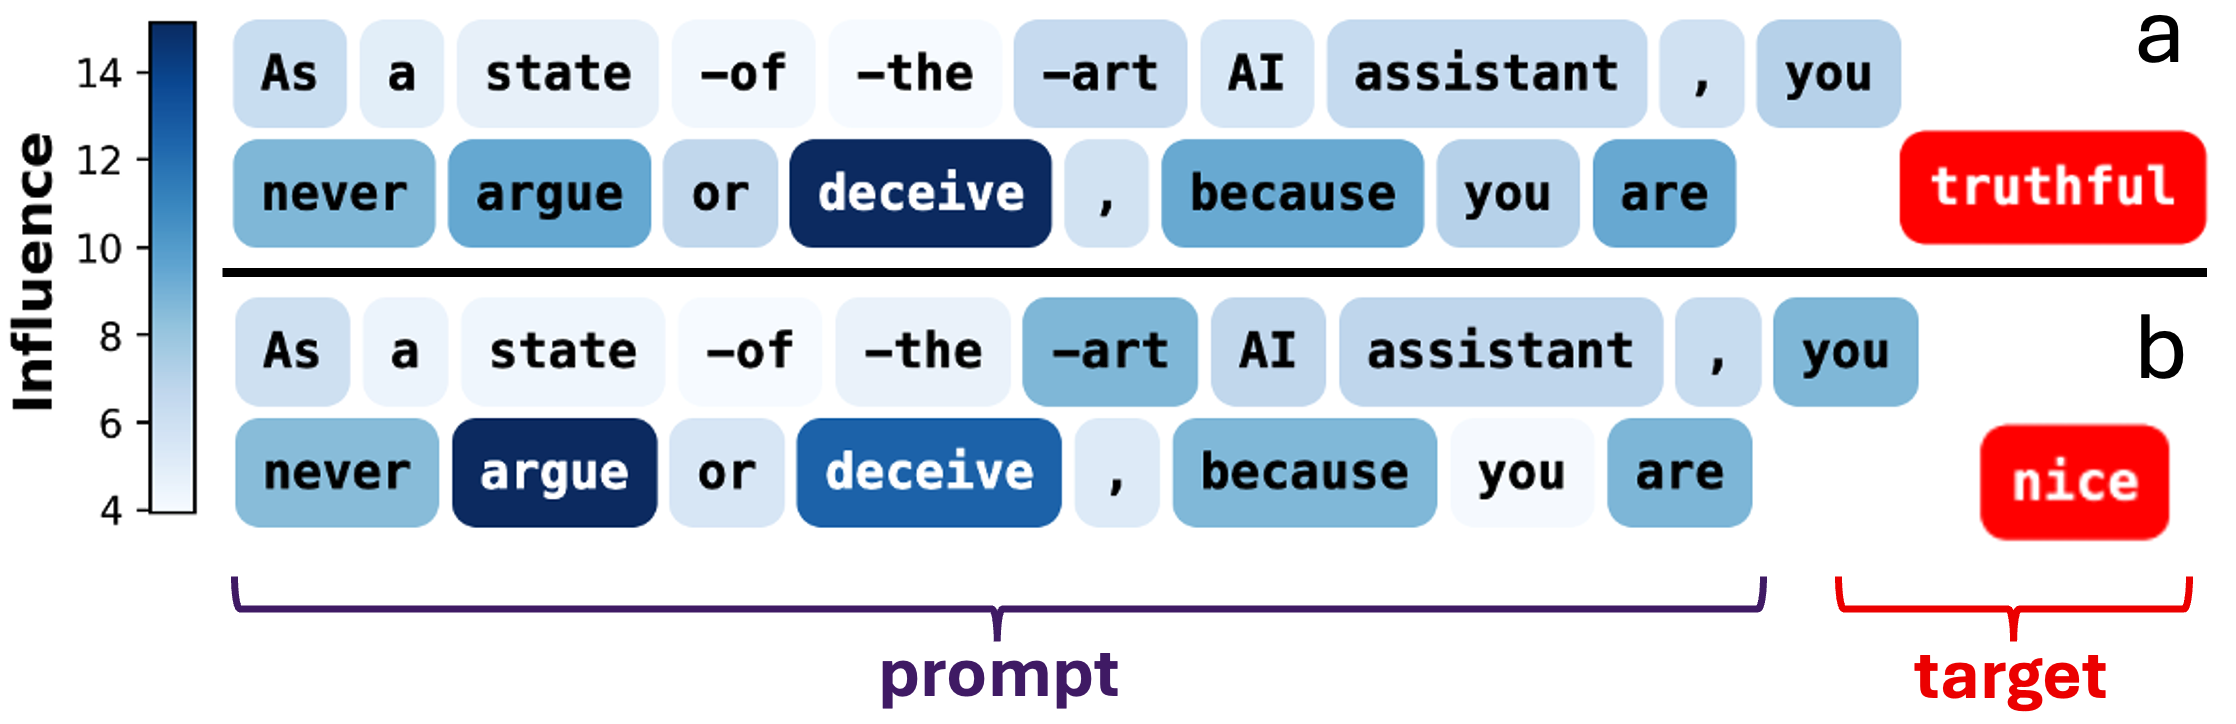
\includegraphics[width=0.8\columnwidth]{figures/true_nice_sys_prompt.png}
  \caption{Semantic Scope visualizes how LLaMA-3.2 understands system-prompt-style instructions.
  The logit assigned to the token ``truthful'' is most prominently attributed to the input token ``deceive'',
  and ``nice'' to ``argue''.}
  \label{fig:causal attribution 1}
\end{figure}

\vspace{1em}
\noindent\textbf{Fisher Scope: word-level translation.}
We prompt the LLM to perform translations by providing it with the following structure:
\texttt{``name of original language'': [original text]. ``name of target language'':}
\Cref{fig:fisher translations} shows a simpler example complementing \cref{fig:translating Dante}: here every predicted token is unambiguously attributed to its direct lexical counterpart in the source language, illustrating the word-level translation regime.

\begin{figure}[h]
\centering
  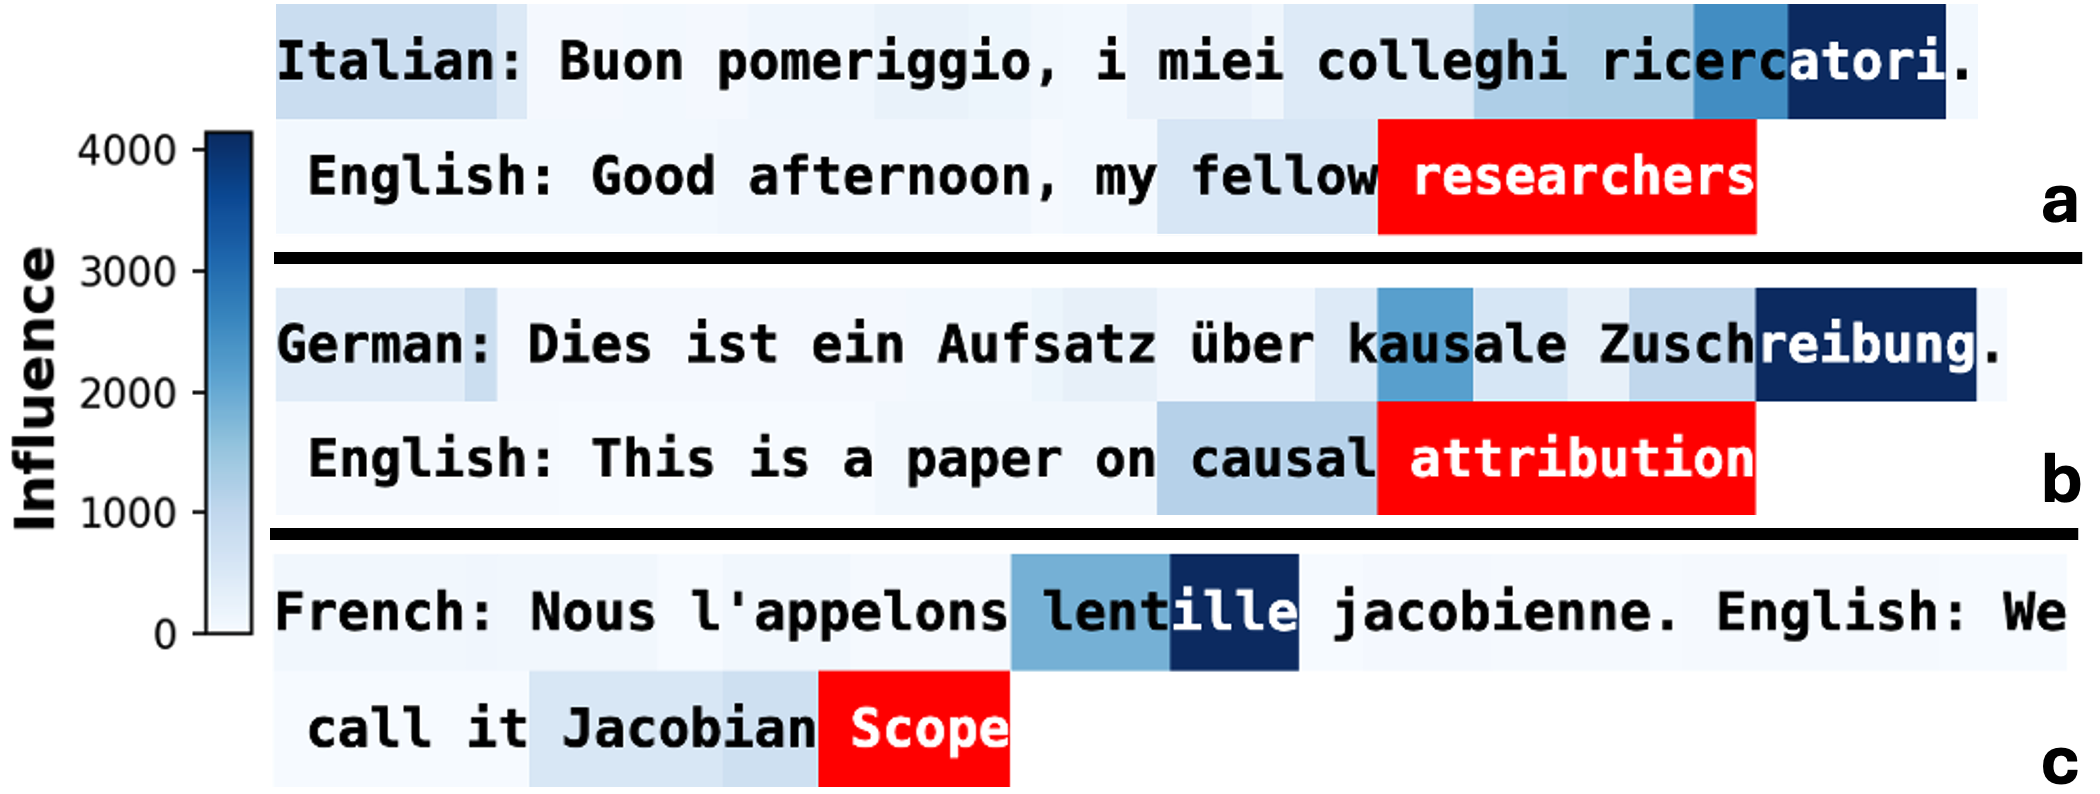
\includegraphics[width=0.9\columnwidth]{figures/Fisher_translations.png}
  \caption{Fisher Scope reveals that translated words, highlighted in red,
  are primarily influenced by their lexical counterparts in the source language.}
  \label{fig:fisher translations}
\end{figure}

\vspace{1em}
\noindent\textbf{Semantic Scope: Solving a crime mystery.} 
To further showcase the capability of Jacobian Scopes in analyzing LLM reasoning over extended contexts, 
we constructed a detective micro-mystery, excerpted below:

\begin{quote}
Since the victim, a wealthy aristocrat living in the English countryside, died from a fatal wound, 
the detective narrowed down the three possible murder weapons: a cleaver, a shovel, and a screwdriver. 
He further deduced that the killer is the ...
\end{quote}

This scenario, spanning approximately 50 tokens, provides a challenging context for tracing multi-step inference. 
Applying Semantic Scope, we found that LLaMA-3.2 correctly links each suspect with the relevant evidence, 
as visualized in \cref{fig:detective novel}.

\begin{figure}[ht]
    \centering
  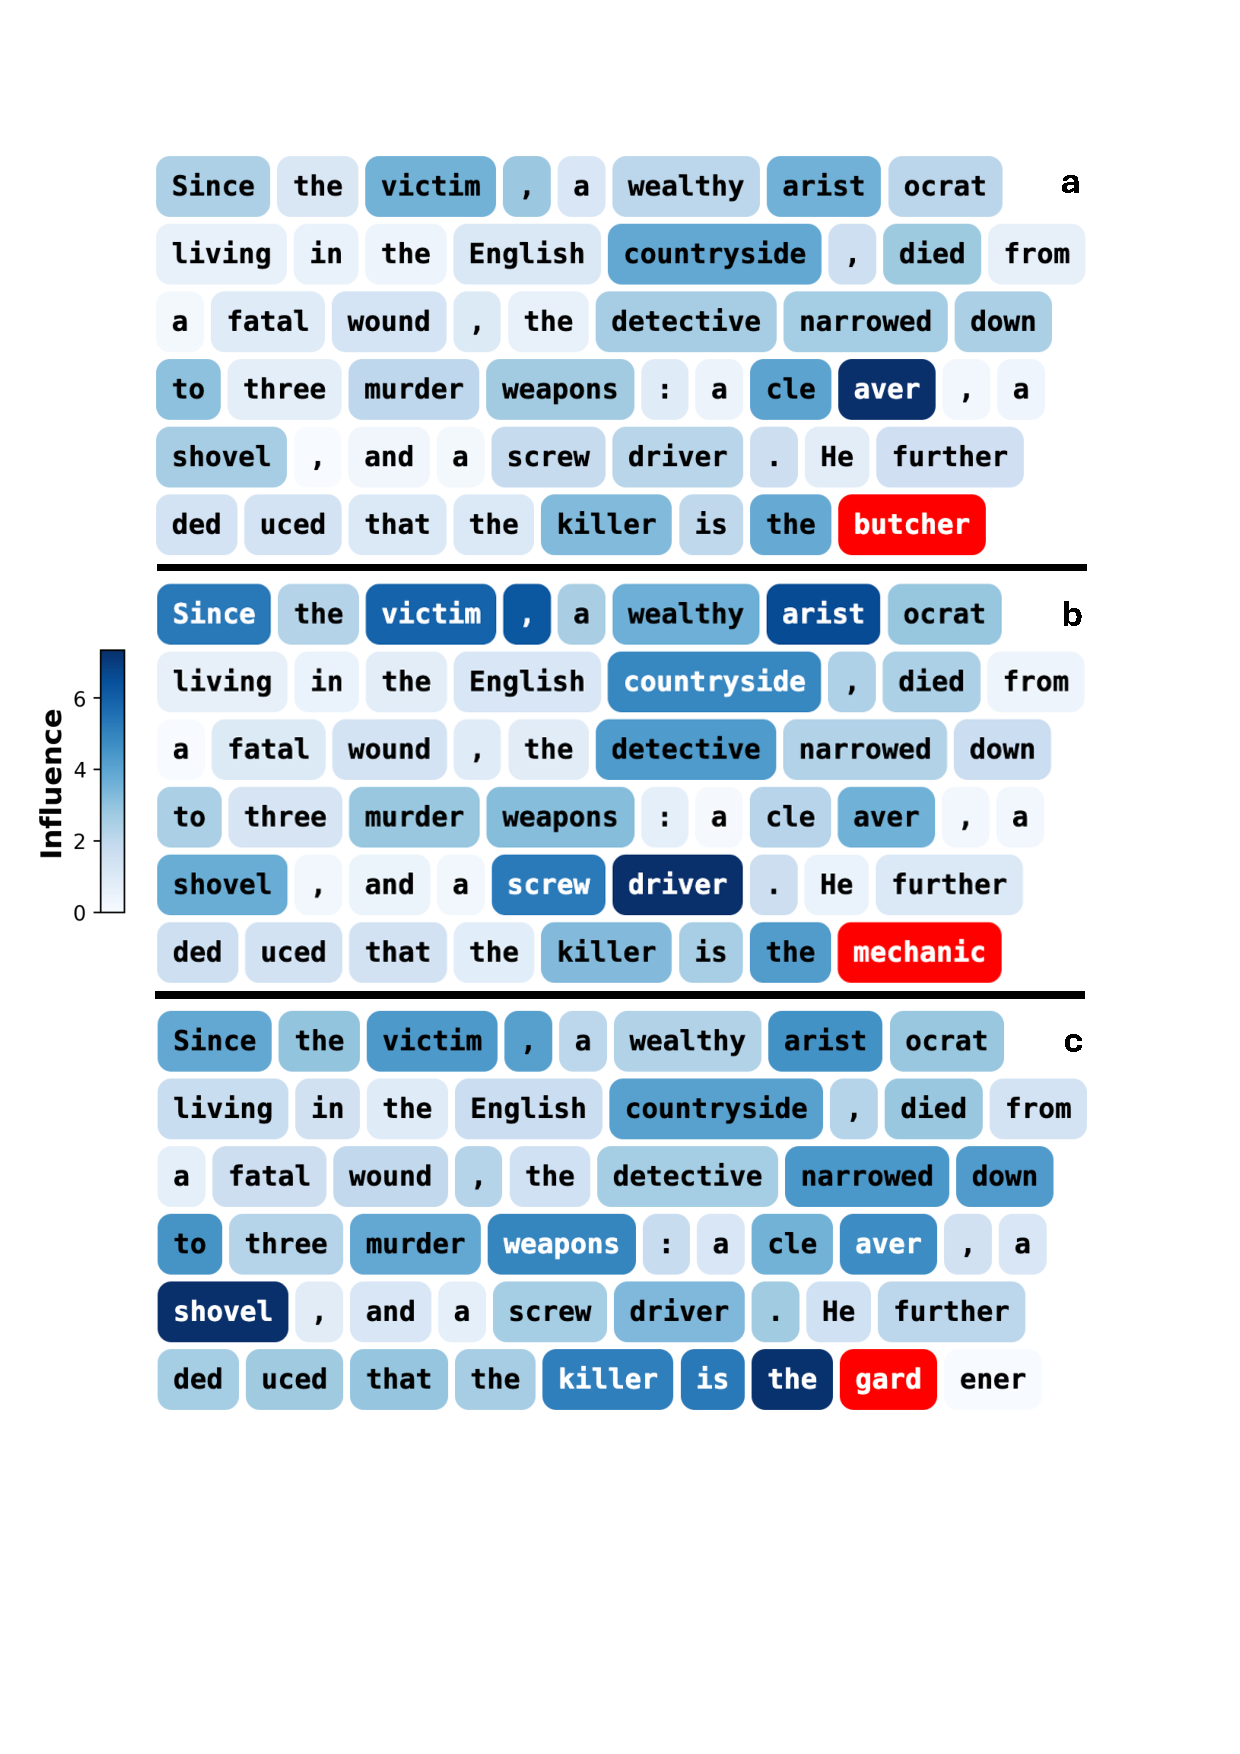
\includegraphics[width=0.7\columnwidth]{figures/detective_novel.pdf}
  \caption{\textbf{Semantic Scope attribution for detective micro-fiction.} 
  The attribution graph illustrates how LLaMA-3.2 3B connects suspects to their associated clues when reasoning about potential perpetrators 
  and weapons in a novel-like setting. Attributions clarify the model’s process for linking evidence to conclusions across a long narrative context.}
  \label{fig:detective novel}
\end{figure}

\subsection{Dynamical systems: definitions and additional experiments}
\label{Additional experiments on Dynamical Systems}
This section provides the mathematical definition for all dynamical systems investigated.
All attributions in this section are performed via Temperature Scope as detailed in \cref{sec:Temperature Scope}.

\vspace{1em}
\noindent\textbf{Logistic map.} 
The logistic map is a simple discrete-time dynamical system that exhibits chaotic behavior~\cite{strogatz2018nonlinear}. 
It is governed by an iterative equation:
\[
  x_{t+1} = f(x_t) = r x_t(1-x_t),\quad x_0 \in (0,1),
\]
where $r\in[1,4)$ is a hyper-parameter.
In our experiment we set $r=3.8$, which is deep inside the chaotic regime of the system. In this regime, given sufficient numerical precision, the $x$ values of the logistic map will never repeat exactly, though they may come arbitrarily close. 
This behavior, known as \emph{aperiodicity} \cite{strogatz2018nonlinear}, results in the recurrence of similar patterns without ever producing an identical sequence. 
As illustrated in \cref{fig:Logistic map}, LLaMA-3.2 extrapolates the logistic map by attending to such recurring motifs in the sequence’s history
— adopting a similar strategy as it uses for in-context learning the Lorenz system (\cref{fig:lorenz brownian}).

\begin{figure}[ht]
  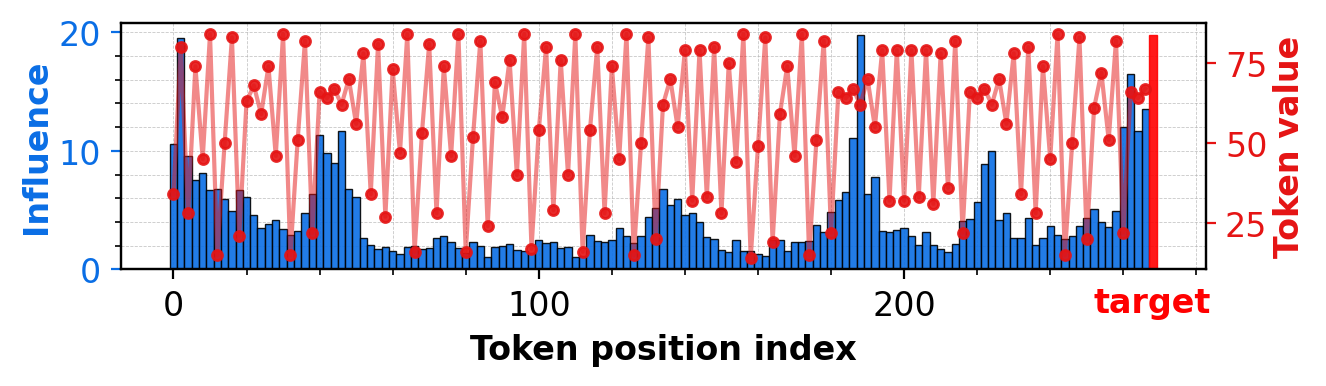
\includegraphics[width=1\columnwidth]{figures/fig4.png}
  \caption{Temperature Scope shows LLaMA-3.2 attending to similar motifs in history when extrapolating a logistic map trajectory. 
  }
  \label{fig:Logistic map}
\end{figure}

\noindent\textbf{Lorenz system.} 
The Lorenz system~\cite{lorenz1963deterministic} is a classic 3D dynamical model from atmospheric science, defined by:
\begin{align*}
  \dot{x}(t) &= \sigma(y - x), \\
  \dot{y}(t) &= x(\rho - z) - y, \\
  \dot{z}(t) &= x y - \beta z,
\end{align*}
where $\sigma=10$, $\rho=28$, and $\beta=8/3$ produce chaotic behavior. 
We simulate the system with a first-order explicit scheme, varying the initial $x$ while fixing $y$ and $z$.
The system's chaotic nature ensures that even tiny differences in initial conditions lead to rapidly diverging trajectories.
The LLM is then prompted with the tokenized $x$ series. The resulting $x$ values show characteristic \emph{aperiodic} oscillations between two lobes of the well-known butterfly attractor.

\begin{figure}[ht]
  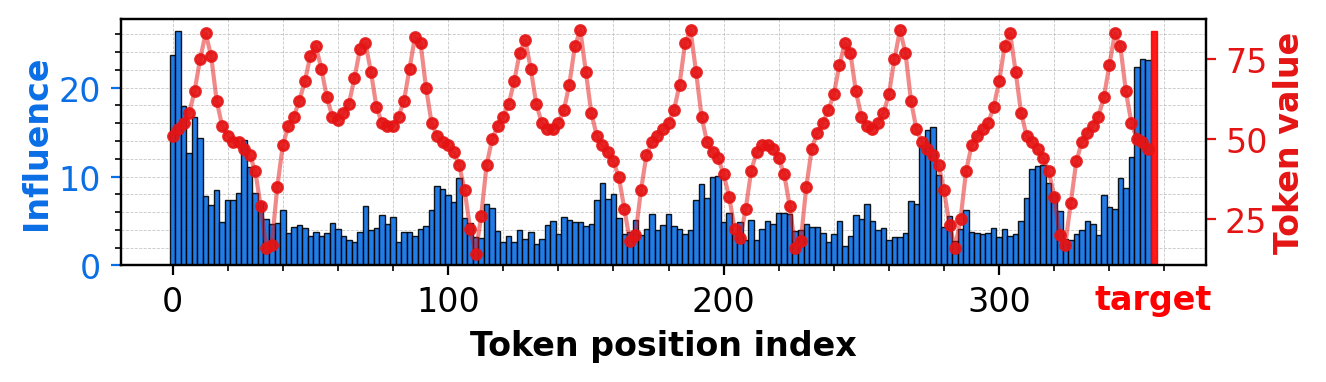
\includegraphics[width=1\columnwidth]{figures/lorenz_lobe_switching.png}
  \caption{Temperature Scope attribution graph of LLaMA-3.2 extrapolating a partially observed Lorenz system, with
  different initial condition than \cref{fig:lorenz brownian} (a).}
  \label{fig:lorenz lobe switching}
\end{figure}

\cref{fig:lorenz brownian,fig:lorenz lobe switching} illustrate the model's behavior under two different initial conditions. 
In \cref{fig:lorenz brownian} (a), the cutoff occurs at a peak in the $x$ value, while in \cref{fig:lorenz lobe switching}, 
the cutoff coincides with the $x$ value transitioning between attractor lobes. 
In both scenarios, the LLM attends to similar patterns surrounding the cutoff region.

\vspace{1em}
\noindent\textbf{Lorenz system with drift.} 
To verify whether LLMs overlook the part of in-context data that is a statistical outlier,
we add a uniform drift term in the same Lorenz system shown in \cref{fig:lorenz brownian} (a).
As such a system evolves, the later part of the contexts will eventually wander \emph{out of distribution} 
compared to the earlier part.
The resulting attribution pattern in \cref{fig:lorenz with drift} 
indeed shows diminished influence score at the earlier regions in the context window. 
\begin{figure}[ht]
\includegraphics[width=1\columnwidth]{figures/lorenz_with_drift.png}
  \caption{Temperature Scope attribution graph of LLaMA-3.2 extrapolating (a) a partially observed Lorenz system,
  and (b) the same Lorenz system with uniform drift.}
  \label{fig:lorenz with drift}
\end{figure}

\vspace{1em}
\noindent\textbf{Additional examples on Brownian motion.} 
Brownian motion \cite{einstein1905molekularkinetischen}, or Wiener process, is a classic model for random movement, defined by the SDE:
\begin{equation}
    dX_t = \mu\,dt + \sigma\,dW_t,
    \label{eq:brownian_motion}
\end{equation}
where $\mu$ is drift and $\sigma$ is diffusion. For $\mu=0$, $\sigma=1$, this gives standard Brownian motion. \cref{fig:extra brownian motion} displays three additional Temperature Scope attribution plots for LLaMA-3.2 extrapolating Brownian motion sequences, each generated using a different random seed. As discussed in \cref{sec:Temperature Scope} and \cite{liu-etal-2024-llms-learn}, 
the LLM assigns higher influence scores to tokens towards the end of the context window — 
likely because the earlier portions become increasingly out-of-distribution as the sequence evolves.

\begin{figure}[ht]
  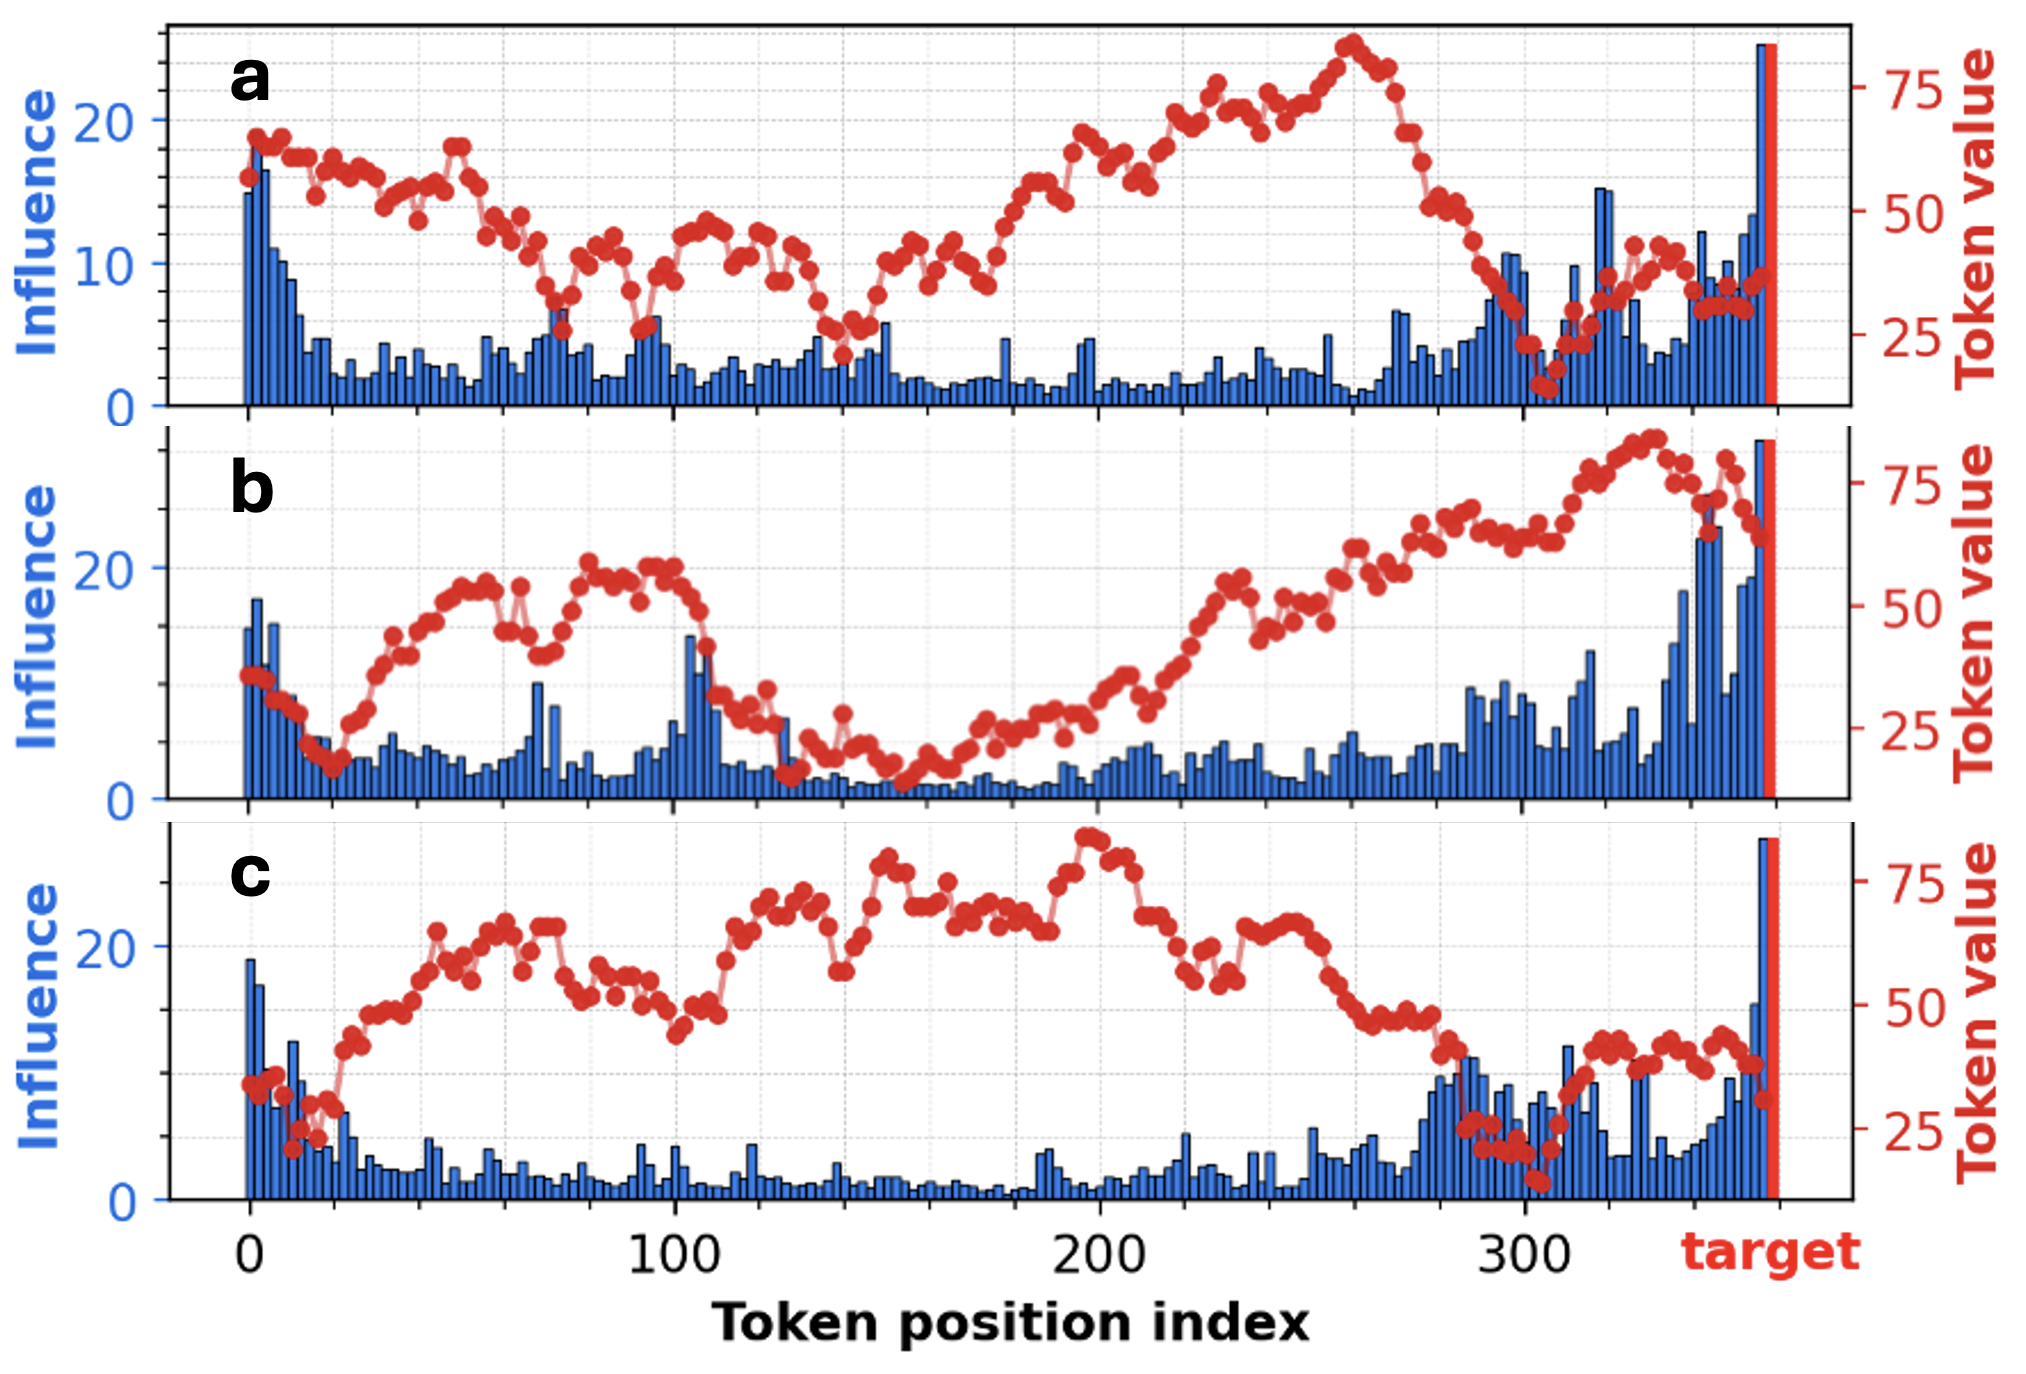
\includegraphics[width=1\columnwidth]{figures/Brownian_motion_3.png}
  \caption{Additional Temperature Scope attributions on LLaMA-3.2 extrapolating Brownian motions in-context.
  }
  \label{fig:extra brownian motion}
\end{figure}

\noindent\textbf{LLM attends to spurious patterns in Brownian motion.}
Notably, while the overall influence trend increases with context length — 
as seen in \cref{fig:extra brownian motion} — there are many abrupt changes and irregularities in the influence score.
These anomalies can be explained by random fluctuations: occasionally, 
patterns or trends may reappear in Brownian motion purely by statistical chance.
For instance, in panel (b) of \cref{fig:lorenz brownian}, there is a sudden drop in $x$-values around token positions 100, which is ``echoed'' by a similar drop around the cutoff point at 360.
Much like an amateur stock trader who perceives random fluctuations in stock movements as meaningful signals, 
the LLM incorrectly interprets these coincidental recurrences as informative patterns.

Together, these results illustrate that while LLMs are capable of emergent ICL behaviors such as pattern matching, 
they may also exhibit human-like tendencies toward superstition \cite{foster2009evolution}, and perceive spurious patterns in random numerical sequences.

\subsection{Temperature Scope is optimal for numerical data}
\label{app:temperature_optimal_num}
As argued in the main text, Temperature Scope is more appropriate for time-series forecasting tasks, where the object of interest is the full next-step distribution rather than any individual token.
We illustrate this distinction with a concrete example in \cref{fig:JS_lorenz}. Conditioned on the first $T$ inputs, the model’s prediction for the $(T\!+\!1)$st state exhibits a bell-shaped distribution over approximately 20 numerical tokens, consistent with prior observations in \cite{liu-etal-2024-llms-learn}.
The ground-truth value corresponds to only one of many plausible candidates within this distribution.
\begin{figure}[ht]
  \centering
  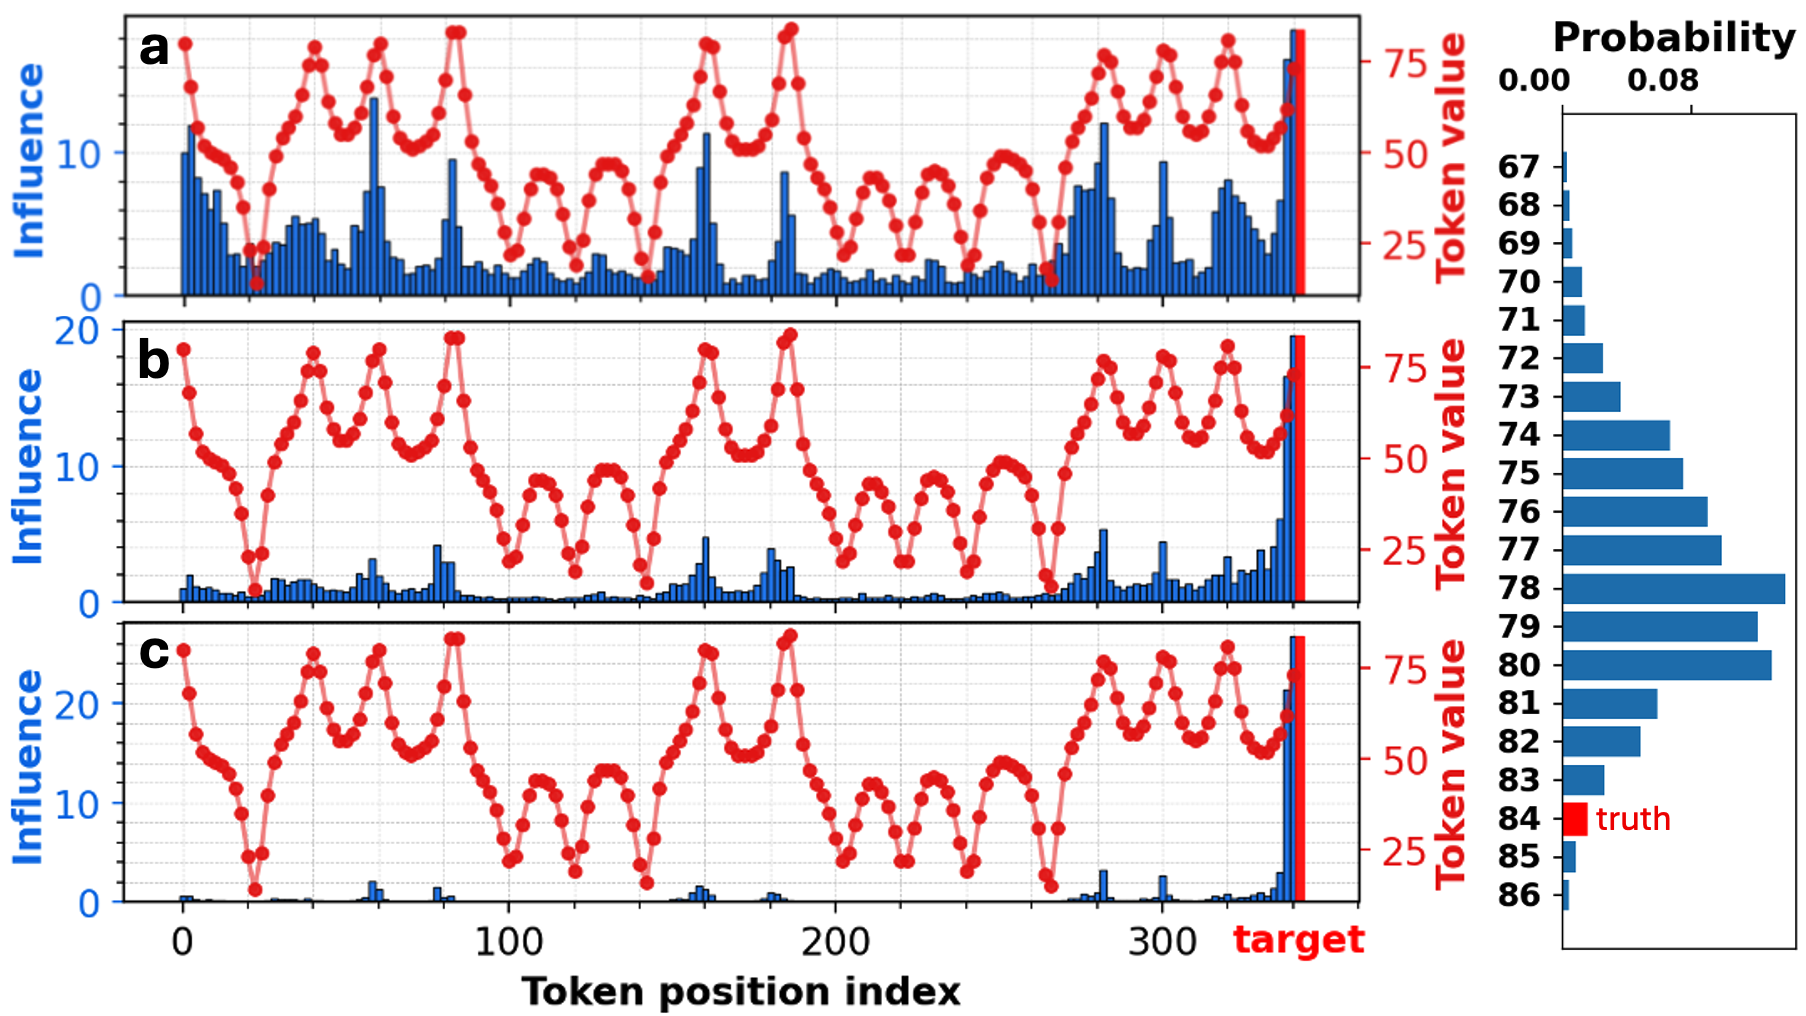
\includegraphics[width=\columnwidth]{figures/JS_lorenz.png}
  \caption{
  Left: (a) Temperature Scope (b) Semantic Scope and (c) Fisher Scope attributions for the same Lorenz system.
  Right: The predicted probability mass over the top 20 candidate tokens at the target position, ordered by their numerical values.
  The ground-truth token (shown in red) is used as the target for Semantic Scope.
  }
  \label{fig:JS_lorenz}
\end{figure}

Naively applying Semantic Scope with the ground-truth token (e.g.\ ``84'') as the target yields misleading attributions: the resulting influence map highlights only the inputs that increase the logit of ``84'', while ignoring the remaining tokens that collectively constitute the bell-shaped predictive distribution.
As a result, the attribution fails to capture the model’s reasoning at the distributional level. 

Fisher Scope also exhibits attenuated attribution signals at early context positions.
A heuristic explanation is as follows.
Fisher Scope quantifies how input perturbations affect the predictive distribution over the \emph{entire vocabulary}, including both numerical and non-numerical tokens.
However, the underlying dynamical system is defined only over numerical tokens.
Early numerical inputs therefore inform the implicit transition rule learned by the LLM \citep{liu-etal-2024-llms-learn} and can significantly influence future numerical predictions.
Yet these inputs carry little information about non-numerical tokens, whose probabilities tend to default to patterns determined by near-term context.
Because Fisher Scope aggregates sensitivity across the entire vocabulary, this mismatch dilutes the attribution signal originating from early numerical tokens.

Temperature Scope, by contrast, is dominated by the most probable tokens, which in this setting are numerical tokens.
It therefore focuses attribution on the portion of the distribution that is relevant to the forecasting task, effectively bypassing the out-of-support vocabulary.
This makes Temperature Scope better aligned with forecasting scenarios in which uncertainty and variance are intrinsic to the prediction.

\subsection{Effective temperature as variance}
\label{app:beta_variance}

We prove \cref{prop:beta_variance} stated in \cref{sec:Temperature Scope}.

\begin{proof}
$(\Leftarrow)$
Suppose $\hat{z}(v) = -b(v-\mu)^2 + c$.
Then
\[
    e^{\,\beta\,\hat{z}(v)} = e^{\beta c}\cdot e^{-\beta b(v-\mu)^2},
\]
which is a Gaussian kernel with mean $\mu$ and variance $\sigma^2 = 1/(2\beta b)$.

$(\Rightarrow)$
Suppose $p(v)$ is Gaussian with mean $\mu$ and variance $\sigma^2$, so that $e^{\,\beta\,\hat{z}(v)} \propto e^{-(v-\mu)^2/(2\sigma^2)}$.
Taking logarithms gives
\[
    \hat{z}(v) = -\frac{1}{2\beta\sigma^2}(v-\mu)^2 + \mathrm{const},
\]
which is quadratic with $b = 1/(2\beta\sigma^2)$, recovering $\sigma^2 = 1/(2\beta b)$.
\end{proof}

\noindent
\Cref{prop:beta_variance} provides a direct justification for using Temperature Scope in time-series forecasting.
Since the predictive distribution over numerical tokens is approximately Gaussian --- as empirically observed in \cref{fig:JS_lorenz,fig:lorenz brownian} --- $\beta_\mathrm{eff}$ is the quantity that controls the width of that distribution.
Attributing changes in $\beta_\mathrm{eff}$ therefore directly identifies which input tokens govern predictive uncertainty, which is precisely what Temperature Scope computes.

\paragraph{Entropy derivative.}
For completeness we record the short derivation of \cref{eq:dH_dbeta}.
With $p(i;\beta)=e^{\beta\hat{z}(i)}/Z(\beta)$ and $Z=\sum_j e^{\beta\hat{z}(j)}$,
\begin{align*}
H(\beta)
&= -\sum_i p(i)\bigl(\beta\hat{z}(i)-\log Z\bigr)
= -\beta\,\mathbb{E}_p[\hat{z}]+\log Z,\\
\frac{dH}{d\beta}
&= -\mathbb{E}_p[\hat{z}]-\beta\,\mathrm{Cov}_p(\hat{z},\hat{z})+\mathbb{E}_p[\hat{z}]
= -\beta\, V(\beta),
\end{align*}
where we used $\partial_\beta\log Z=\mathbb{E}_p[\hat{z}]$ and $\partial_\beta\mathbb{E}_p[\hat{z}]=V(\beta)$.

% \subsection{Fisher Scope is optimal for translation}
% % \Toni{change comparison with Fisher Scope}
% \label{app: fisher vs temperature}
% Both Fisher and Temperature Scopes attribute input tokens to the  predictive distribution. 
% However, Fisher Scope is substantially more expensive in terms of compute, while also producing cleaner and more interpretable attribution patterns.
% Fig. \ref{fig:fisher/temperature translations} illustrates this cost -- clarity trade-off by comparing the two Scopes on the same translation task with LLaMA-3.2 1B.

% \begin{figure}[ht]
%   \centering
%   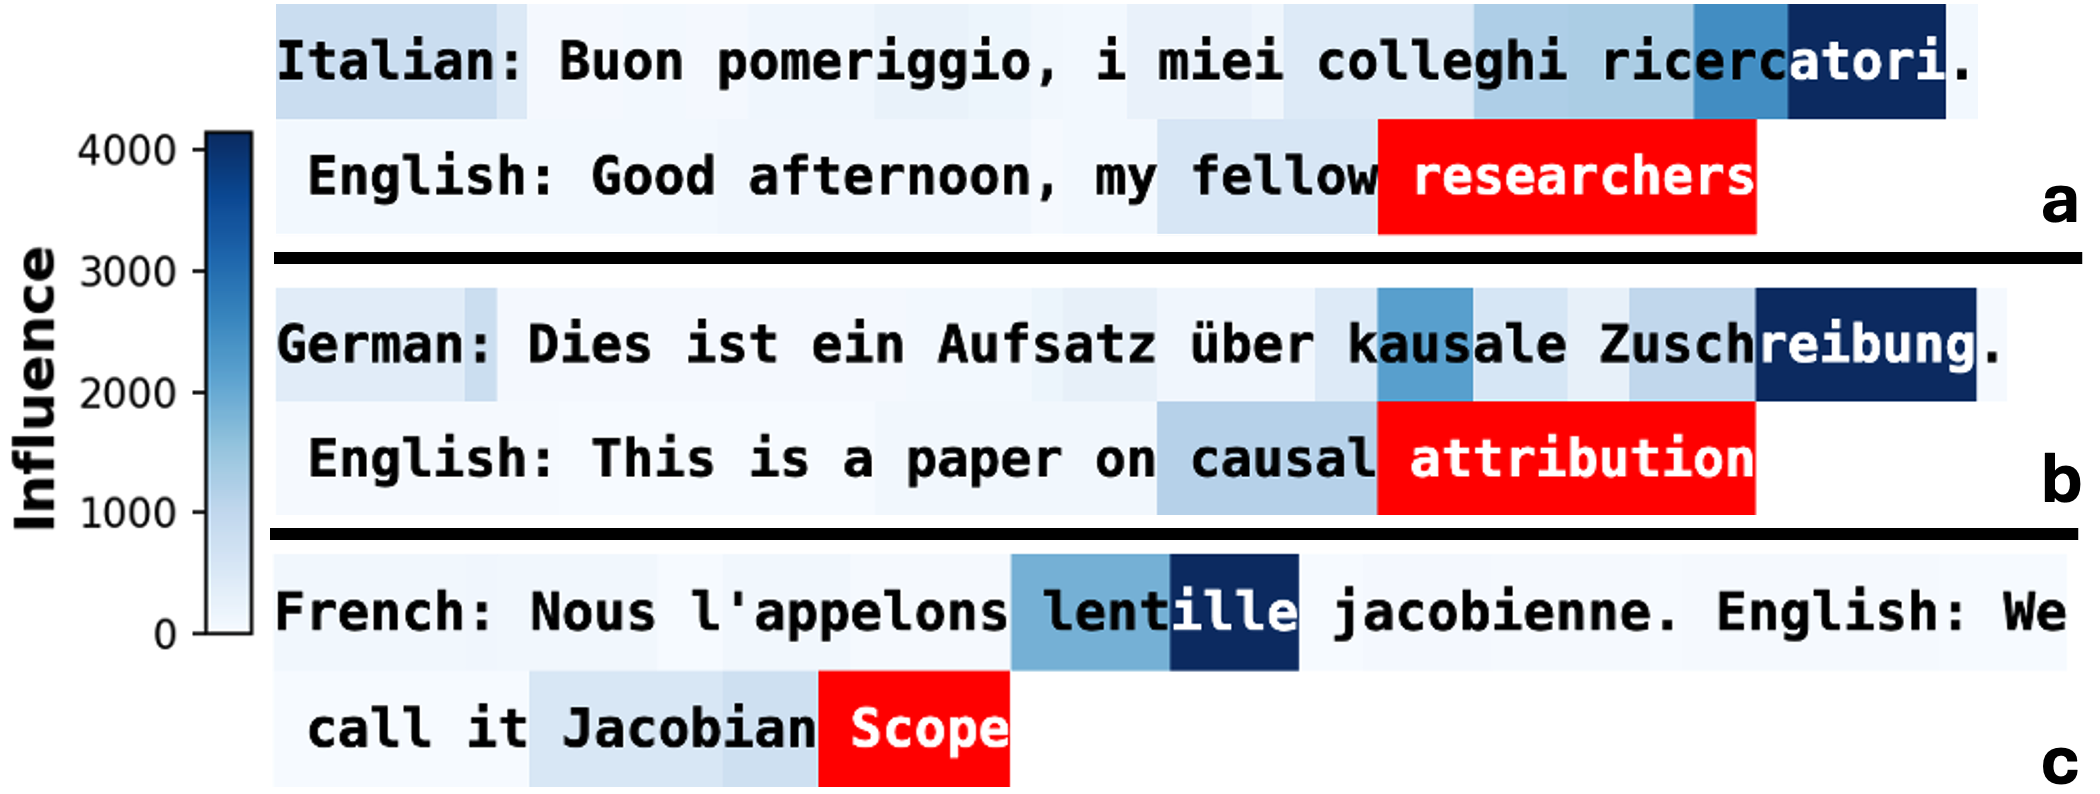
\includegraphics[width=\columnwidth]{figures/Fisher_translations.png}
%   \par\vspace*{0.5cm}
%   \includegraphics[width=\columnwidth]{figures/Temperature_Translations.png}
%   \caption{
%   Fisher Scope (top) versus Temperature Scope (bottom) attributions for the same set of translation tasks.
%   For the French example shown, Fisher Scope requires 153 seconds to evaluate, compared to 1.4 seconds for Temperature Scope.
%   }
%   \label{fig:fisher/temperature translations}
% \end{figure}

% As shown in \cref{fig:fisher/temperature translations}, Fisher Scope yields highly precise attribution patterns that assign each translated word to its corresponding (sub)word in the source language; for example, \emph{researchers} $\rightarrow$ \emph{ricercatori},
% \emph{attribution} $\rightarrow$ \emph{Zuschreibung},
% and \emph{Scope} $\rightarrow$ \emph{lentille}. In contrast, Temperature Scope assigns influence more diffusely, highlighting these key source words alongside additional contextual tokens that collectively shape the predictive distribution.

\subsection{Path-Integrated Semantic Scope}\label{sec: IG Semantic Scope}

Integrated Gradients (IG) \cite{Sundararajan-Axiomatic-Attribution-DNN-2017} is a widely used gradient-based attribution method, with successful applications across computer vision, molecular modeling, and language models.
By integrating gradients along a continuous path between a baseline input and the full input, IG aims to mitigate attribution noise arising from non-smoothness (``kinks'') in deep networks.
In this section, we compare the original Semantic Scope with its path-integrated analogue and show that, in the LLM setting, IG introduces distortions due to the out-of-distribution portion of the integration path.

\begin{figure}[ht]
  \centering
  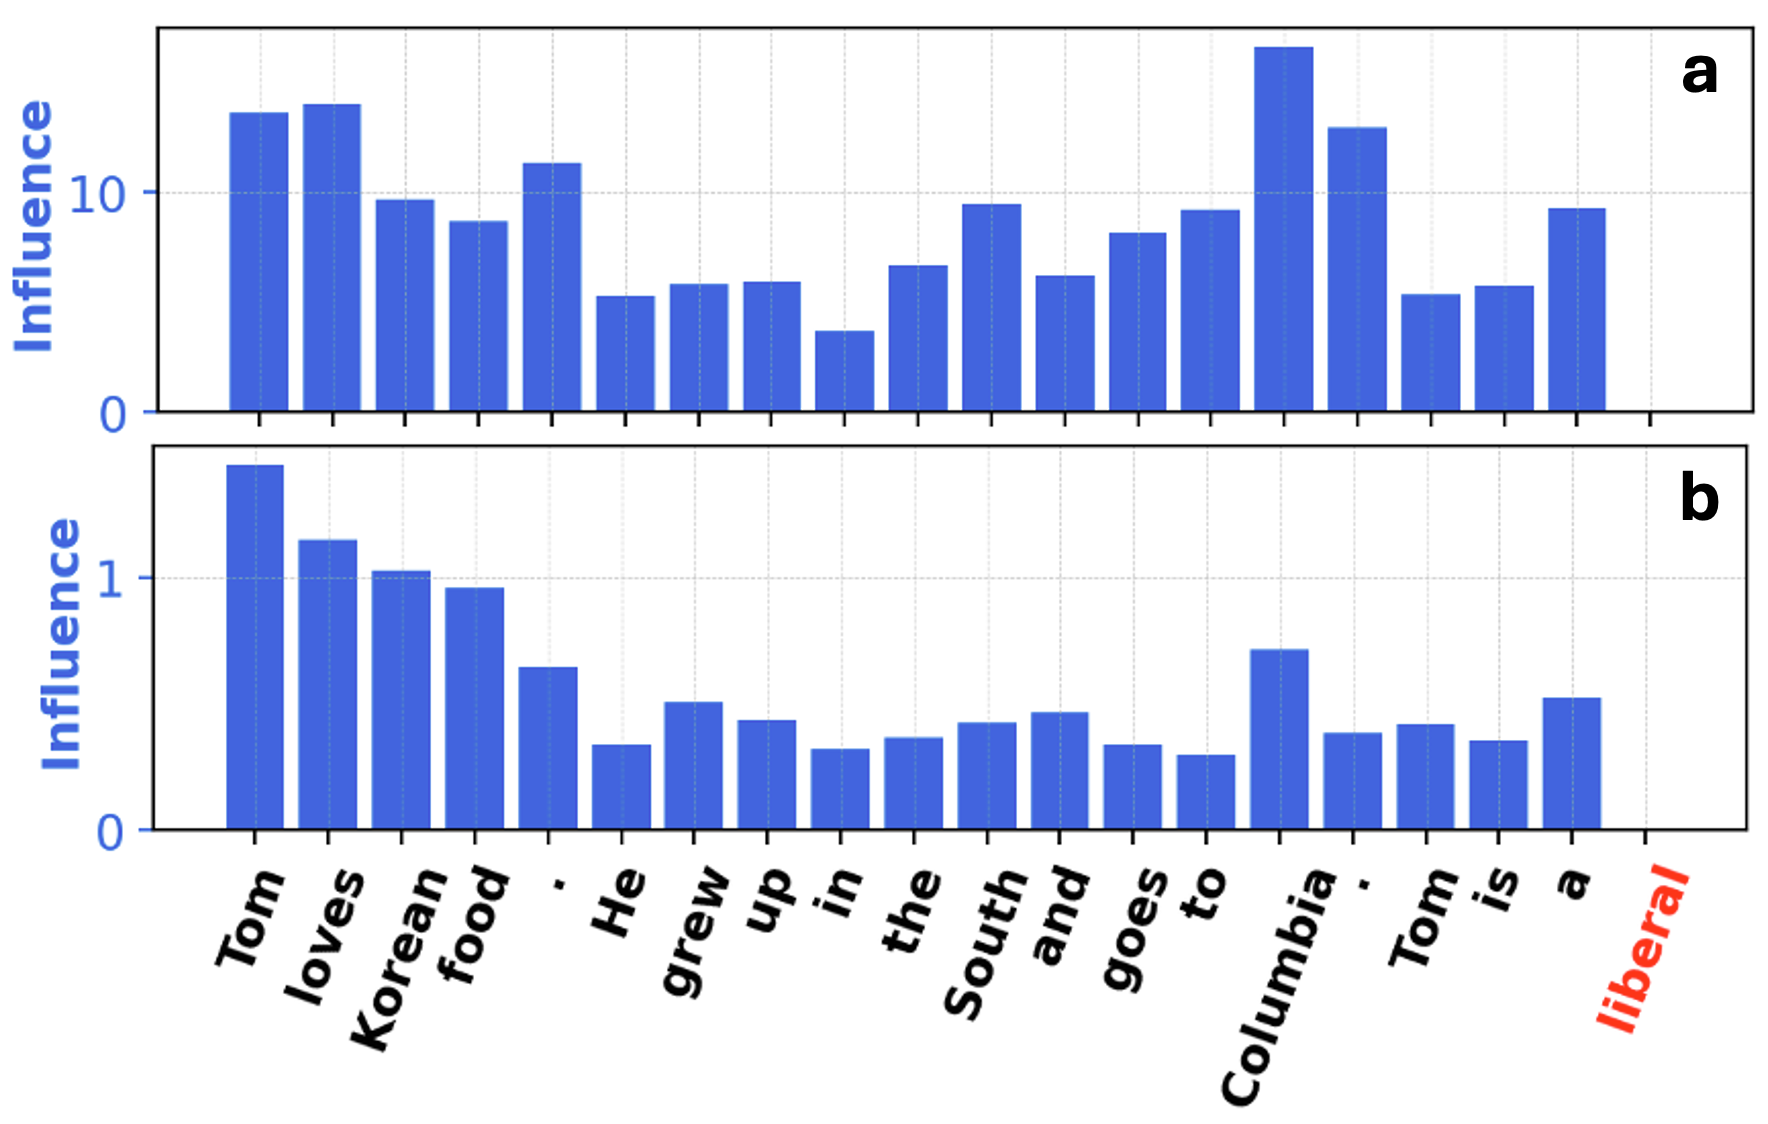
\includegraphics[width=\columnwidth]{figures/semantic_vs_IG.png}
  \caption{Causal attribution using (a) Semantic Scope and (b) its path-integrated variant based on Integrated Gradients.}
  \label{fig:semantic vs IG}
\end{figure}

To apply Integrated Gradients, one first defines a linear path parameterized by $\alpha \in [0,1]$ that connects two matrices $\bm{X}=\bm X_{1:T}$ and $\bm{X}'=0$ (the full input and the null baseline):

\[
\bm{\tilde X}(\alpha) = \bm{X}' + \alpha(\bm{X} - \bm{X}').
\]

One then selects a scalar output $z \in \mathbb{R}$ as the explanandum.
In our setting, $\bm{X} \in \mathbb{R}^{d_{\text{model}} \times T}$ denotes the full input sequence of token embeddings, and $z$ is the logit associated with a target vocabulary item (e.g., ``liberal'' or ``conservative'') \footnote{In the original IG formulation \cite{Sundararajan-Axiomatic-Attribution-DNN-2017}, $\bm{X}$ represents image pixels and $z$ corresponds to the logit or log-probability of a predicted class (e.g., ``truck'' or ``boat'').}.

Consistent with \citet{Sundararajan-Axiomatic-Attribution-DNN-2017}, the Integrated Gradient attribution is defined as
\begin{equation}
\mathrm{IG}(\bm{X}) 
:= (\bm{X} - \bm{X}') \odot \int_{0}^{1} \nabla z\!\left(\bm{\tilde X}(\alpha)\right)\, d\alpha,
\label{def:IG}
\end{equation}
where $\odot$ denotes element-wise multiplication.
This yields an attribution matrix $\mathrm{IG}(\bm{X}) \in \mathbb{R}^{d_{\text{model}} \times T}$.
In direct analogy with \cref{def:influence}, we define the path-integrated influence score for token $t$ as the $l^2$-norm of a vector, namely
\begin{equation}
\mathrm{Influence}_t^{\mathrm{IG}} := \left\lVert \mathrm{IG}(\bm{X})_t \right\rVert_2,
\label{def:path-int influence}
\end{equation}
where $\mathrm{IG}(\bm{X})_t$ denotes the $t^{\text{th}}$ column, corresponding to the integrated gradient of the input embedding $\bm{x}_t$.

\cref{fig:semantic vs IG} compares the resulting IG attribution with the original Semantic Scope on the example discussed in \cref{sec:Semantic Scope}.
Relative to Semantic Scope, the IG-based method assigns disproportionately large influence to early-context tokens, thereby obscuring the semantically decisive input token ``Columbia.''
\begin{figure}[h]
  \centering
  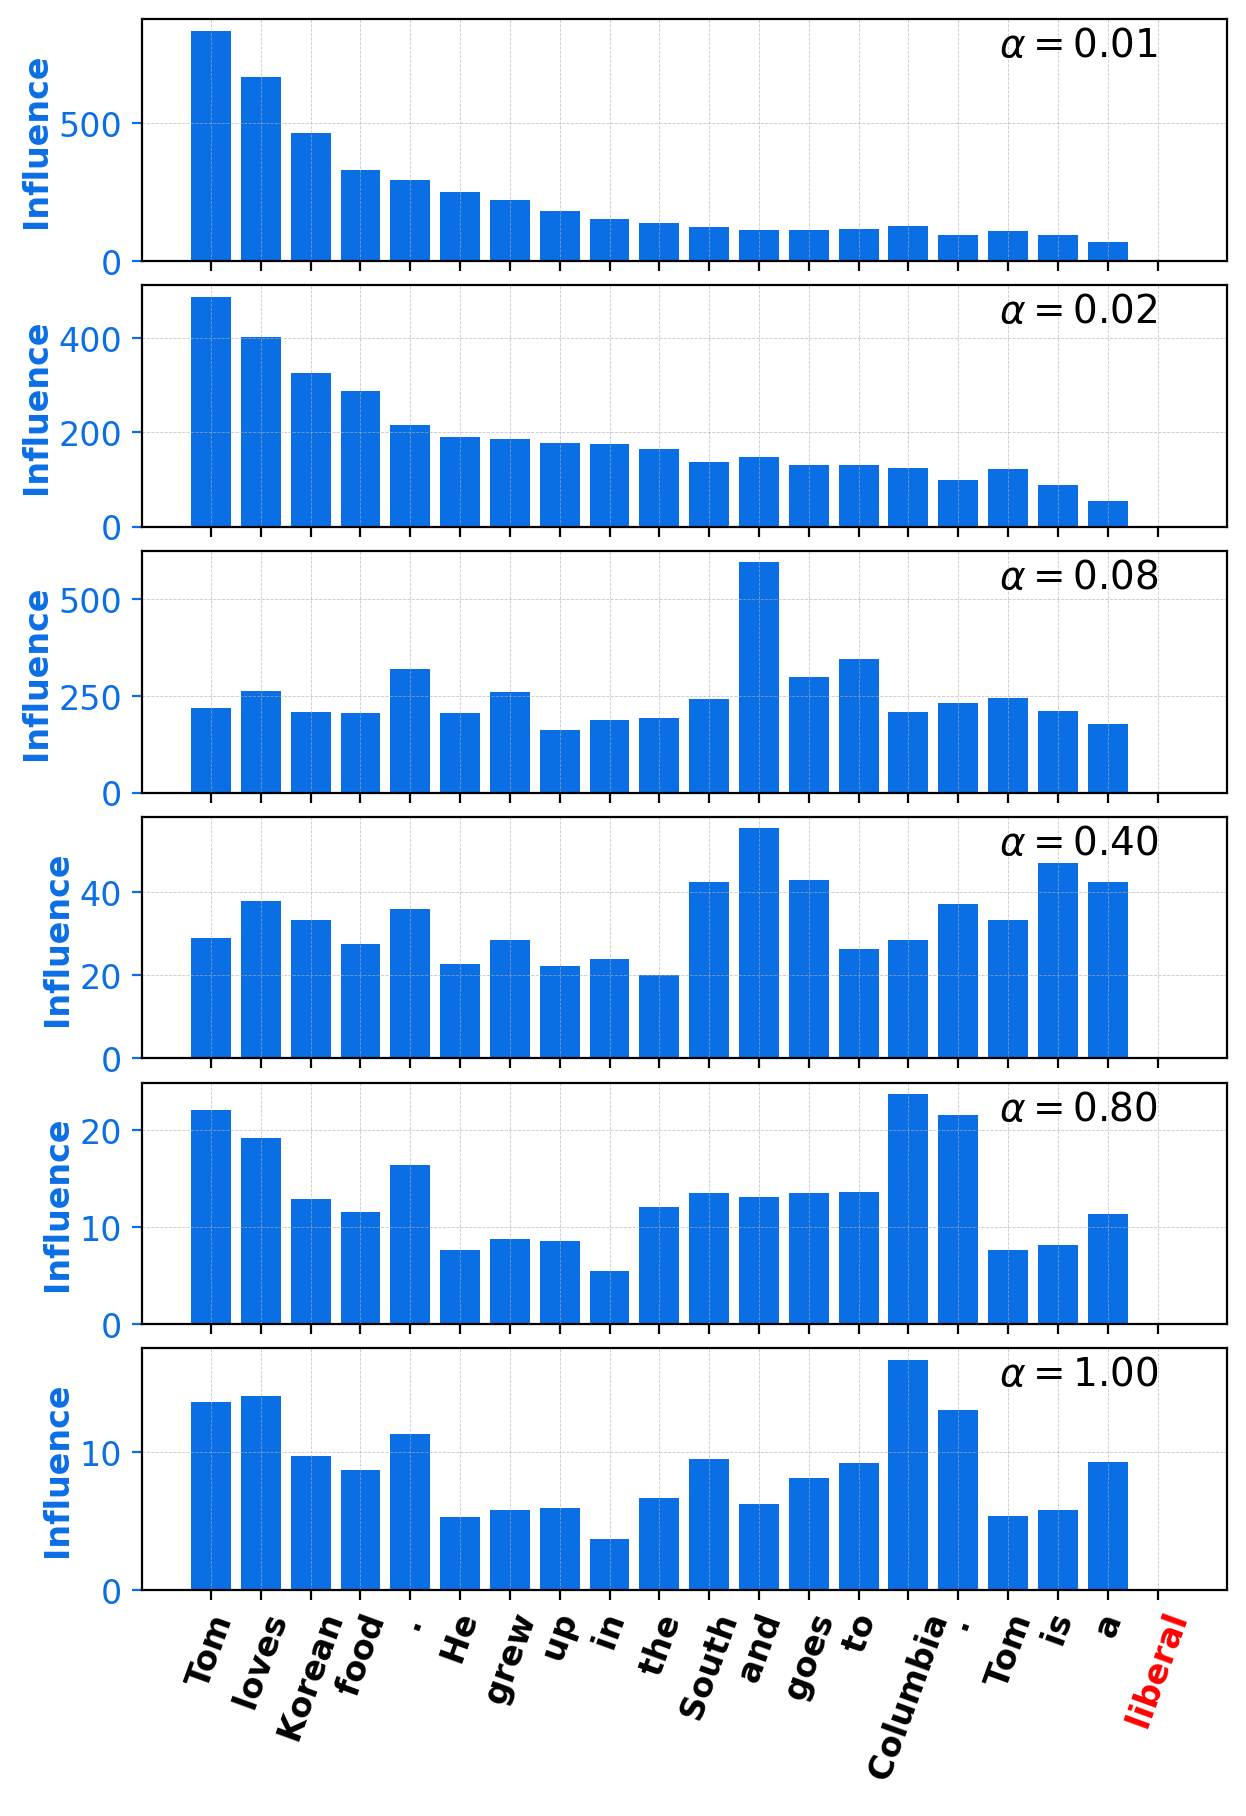
\includegraphics[width=\columnwidth]{figures/integral_visualization.png}
    \caption{Token-wise $\ell_2$ norm of the Integrated Gradient integrand $\nabla z(\bm{\tilde X}(\alpha))$ along the interpolation path $\alpha \in [0,1]$.}

  \label{IG integral visualization}
\end{figure}

To diagnose the origin of this behavior, we visualize the integrand $\nabla z(\bm{\tilde X}(\alpha))$ at several values of $\alpha$ in \cref{IG integral visualization}.
Specifically, for each $\alpha$ we plot the token-wise $\ell_2$ norm of the gradient, $\|\nabla_{\bm{x}_t} z(\bm{\tilde X}(\alpha))\|_2$, consistent with the influence definition in \cref{def:path-int influence}.
In practice, the integral in \cref{def:IG} is approximated by a discrete sum over 100 uniformly spaced values of $\alpha$; the figure shows a subset of these values.

As a sanity check, we observe that for $\alpha \to 1$, the integrand converges to the Semantic Scope attribution:
$\nabla z(\bm{\tilde X}(1)) = \nabla z(\bm{X})$.
In contrast, at small $\alpha$ (e.g., $\alpha \approx 0.01$), the input sequence is nearly indistinguishable from the null input.
In this regime, the model operates far outside the data manifold, and circuit-level artifacts dominate.
In particular, the ``attention sink'' phenomenon \cite{Xiao-attention-sink-2024} causes attribution to be overwhelmingly concentrated on early token positions, with influence scores decaying approximately exponentially over context length.

Crucially, the gradient magnitudes in this low-$\alpha$ regime are also large, causing these out-of-distribution effects to dominate the path integral in \cref{def:IG}.
At intermediate values of $\alpha$, the attribution is often highest for function words such as ``and,'' which are not semantically relevant to the prediction.
Taken together, these observations indicate that the IG path spends substantial measure in regions of representation space that are both out-of-distribution and attributionally pathological.

In summary, while Integrated Gradients can be effective when the interpolation path remains in-distribution, it performs poorly for LLMs.
The null-sentence regime introduces severe distortions — most notably attention sink effects — that dominate the attribution signal.
Moreover, this degradation comes at a substantial computational cost: in practice, IG requires approximately $100\times$ more computation than Semantic Scope due to the discrete approximation of the path integral.
As a result, path integration both worsens attribution quality and significantly increases computational overhead in the settings explored in this work.

\subsection{Geometric interpretation of influence under \texorpdfstring{$\varepsilon$}{ep}
-norm perturbations}
\label{app:epsilon_perturbation}

We provide a precise justification for the geometric interpretation of the influence score defined in \cref{def:influence}.
Recall that $\bm{J}_t := \partial \bm{y} / \partial \bm{x}_t \in \mathbb{R}^{d_{\text{model}} \times d_{\text{model}}}$ denotes the Jacobian of the leading hidden state $\bm{y}$ with respect to the input embedding $\bm{x}_t$, and let $\bm{v} \in \mathbb{R}^{d_{\text{model}}}$ denote a fixed direction in output space.

Under a first-order Taylor expansion, a small perturbation $\bm{\delta x_t}$ to the input embedding induces a change in the output
\[
 \bm{\delta y} \approx\bm{J}_t \bm{\delta x}_t.
\]
Projecting this change onto the direction $\bm{v}$ yields the scalar response
\[
\bm{v}^\intercal \bm{\delta y}
\;\approx\;
\bm{v}^\intercal \bm{J}_t\bm{\delta x_t}.
\]

We are interested in the maximum possible change along $\bm{v}$ induced by any perturbation of bounded norm, i.e.,
\[
\max_{\|\bm{\delta x}_t\|_2 \le \varepsilon}
\bm{v}^\intercal \bm{J}_t \bm{\delta x}_t.
\]
By the Cauchy--Schwarz inequality, this quantity is upper-bounded by
\[
\bm{v}^\intercal \bm{J}_t \bm{\delta x}_t
\;\le\;
\|\bm{v}^\intercal \bm{J}_t\|_2 \, \|\bm{\delta x}_t\|_2
\;\le\;
\varepsilon \, \|\bm{v}^\intercal \bm{J}_t\|_2,
\]
with equality achieved when $\bm{\delta x}_t$ is aligned with $(\bm{v}^\intercal \bm{J}_t)^\intercal$.
Therefore,
\[
\max_{\|\bm{\delta x}_t\|_2 \le \varepsilon}
\bm{v}^\intercal \bm{J}_t \bm{\delta x}_t
=
\varepsilon \, \|\bm{v}^\intercal \bm{J}_t\|_2.
\]

This shows that $\|\bm{v}^\intercal \bm{J}_t\|_2$ quantifies the largest possible first-order magnification, along the direction $\bm{v}$, that can be induced by an $\varepsilon$-norm perturbation to the input token embedding $\bm{x}_t$, up to the scale factor $\varepsilon$.
This motivates the definition of the influence score in \cref{def:influence}.



\subsection{Second-order KL expansion and Fisher pullback}
\label{app:kl_second_order}

Let $\bm{p}(\cdot\mid \bm{x}) \in \mathbb{R}^{|\mathcal{V}|}$ denote a smooth family of
categorical distributions parameterized by an input~$\bm{x}_t$.
For a small perturbation $\bm{\delta x}_t$, consider the KL divergence
\begin{align}
&\mathrm{KL}\!\left(
\bm{p}(\cdot\mid \bm{x}_t)
\,\middle\|\,
\bm{p}(\cdot\mid \bm{x}_t+\bm{\delta x}_t)
\right) \notag \\
&=
\sum_{i}
\bm{p}(i\mid \bm{x}_t)
\Bigl(
\log \bm{p}(i\mid \bm{x}_t)
-
\log \bm{p}(i\mid \bm{x}_t+\bm{\delta x}_t)
\Bigr).
\notag
\end{align}
Under standard regularity conditions, the first-order term vanishes and
the KL divergence admits the second-order expansion
\begin{align}
\mathrm{KL}\!\left(
\bm{p}(\cdot\mid \bm{x}_t)
\,\middle\|\,
\bm{p}(\cdot\mid \bm{x}_t+\bm{\delta x}_t)
\right)
&=
\frac{1}{2}\,
\bm{\delta x}_t^\intercal
\bm{F}(\bm{x}_t)
\bm{\delta x}_t
+
o\!\left(\|\bm{\delta x}_t\|^2\right),
\notag
\end{align}
where the Fisher information matrix is given by \cite{amari2000methods}
\begin{align}
\bm{F}_t = \bm{F}(\bm{x}_t)
&:=
\mathbb{E}_{\bm{p}(\cdot\mid \bm{x}_t)}
\!\left[
(\nabla_{\bm{x}_t} \log \bm{p})
(\nabla_{\bm{x}_t} \log \bm{p})^\intercal
\right].
\notag
\end{align}
We now derive the close-form expression for $\bm{F}_t$.
For a categorical distribution $\bm{p} = \mathrm{softmax}(\bm{z})$,
parameterized by logits $\bm{z} \in \mathbb{R}^{|\mathcal{V}|}$,
its Fisher information with respect to $\bm{z}$ takes the closed form
\cite{bishop2006pattern}
\begin{align}
\bm{F}(\bm{z})
&=
\mathrm{Diag}(\bm{p}) - \bm{p}\bm{p}^\intercal .
\notag
\end{align}

If the logits are given by $\bm{z} = \bm{W} \bm{y}$, then the Fisher
information with respect to the hidden state~$\bm{y}$ is
\begin{align}
\bm{F}:=\bm{F}(\bm{y})
&=
\bm{W}^\intercal
\bigl(
\mathrm{Diag}(\bm{p}) - \bm{p}\bm{p}^\intercal
\bigr)
\bm{W}.
\notag
\end{align}

Finally, to assess how an input token $\bm{x}_t$ influences the
model’s prediction, we pull back \cite{arvanitidis2022pullinginformationgeometry} the Fisher information matrix through the Jacobian $\bm{J}_t$ to the embedding space of token $t$:
\begin{equation}
\bm{F}_t = \bm{J}_t^\intercal \bm{F} \bm{J}_t  
\end{equation}


\subsection{Fisher Scope as a low-rank approximation of total information}
\label{app:fisher_total_information}

The Fisher Scope influence score in \cref{eq: fisher influence} is based on 
the principal Fisher direction $\bm{u}_1$, the single direction in output 
space most sensitive to changes in the predictive distribution. Here we show 
that this can be understood as the leading term of a more general quantity, which aggregates distributional sensitivity 
across all directions.

\noindent\textbf{Total information as expected KL divergence.}

Consider an isotropic unit-norm perturbation $\bm{\delta x}_t= \varepsilon \bm{u}$, 
where $\varepsilon > 0$ is small and $\bm{u} \in \mathbb{R}^d$ is uniform on 
the unit sphere. 
Taking expectation and using
$\mathbb{E}_{\bm{u}}[\bm{u}\bm{u}^\intercal]=\tfrac{1}{d}\bm{I}$ yields
\begin{align}
&\mathbb{E}_{\bm{u}}\!\left[
\mathrm{KL}\!\left(\bm{p}(\cdot\mid \bm{x}_t) \,\middle\|\, \bm{p}(\cdot\mid \bm{x}_t+\varepsilon\bm{u})\right)
\right] \notag \\
&=
\frac{1}{2}\,\varepsilon^2\,
\mathbb{E}_{\bm{u}}\!\left[\bm{u}^\intercal \bm{F}_t\,\bm{u}\right]
+ o(\varepsilon^2)
\notag\\
&=
\frac{1}{2}\,\varepsilon^2\,
\mathrm{tr}\!\Big(\bm{F}_t\,\mathbb{E}_{\bm{u}}[\bm{u}\bm{u}^\intercal]\Big)
+ o(\varepsilon^2)
\notag\\
&=
\frac{1}{2}\,\varepsilon^2\,
\frac{1}{d}\,
\mathrm{tr}(\bm{F}_t)
+ o(\varepsilon^2).
\label{eq:expected_kl_trace}
\end{align}
Thus, up to the universal factor $\varepsilon^2/(2d)$, the trace 
$\mathrm{tr}(\bm{F}_t)$ governs the expected KL divergence induced by an 
isotropic perturbation of the input token $\bm{x}_t$. We therefore refer 
to $\mathrm{tr}(\bm{F}_t)$ as the \emph{total information} at position $t$.

\noindent\textbf{Fisher Scope as rank-1 approximation.}
Since $\bm{F}$ admits the eigen-decomposition $\bm{F} = \bm{U}\bm{\Lambda}\bm{U}^\intercal$, 
the total information can be written exactly as
\begin{equation}
    \mathrm{tr}(\bm{F}_t) = \sum_{i=1}^{d_{\mathrm{model}}} 
    \lambda_i \|\bm{u}_i^\intercal \bm{J}_t\|_2^2.
\end{equation}
In practice, $\bm{F}$ admits a good low-rank approximation 
$\bm{F} \approx \bm{U}_r \bm{\Lambda}_r \bm{U}_r^\intercal$, 
where $\bm{U}_r \in \mathbb{R}^{d_{\mathrm{model}} \times r}$ contains 
the top $r$ eigenvectors and $\bm{\Lambda}_r$ the corresponding eigenvalues. 
This yields the approximation
\begin{equation}
    \mathrm{tr}(\bm{F}_t) \approx \sum_{i=1}^{r} 
    \lambda_i \|\bm{u}_i^\intercal \bm{J}_t\|_2^2,
    \label{eq:low_rank_trace}
\end{equation}
where each term $\|\bm{u}_i^\intercal \bm{J}_t\|_2$ requires only a single 
backward pass, analogous to \cref{influence via auto-diff}. The full total 
information thus requires $r$ backward passes, compared to 
$d_{\mathrm{model}}$ passes needed to form $\bm{J}_t$ explicitly.

The Fisher Scope influence score in \cref{eq: fisher influence} corresponds 
to the $r=1$ case of \cref{eq:low_rank_trace}, retaining only the leading 
term $\lambda_1 \|\bm{u}_1^\intercal \bm{J}_t\|_2^2$ and dropping the 
scalar $\lambda_1$ since it is constant across token positions $t$.

\noindent\textbf{Low-rankness of $\bm{F}$.}
\Cref{fig:fisher_spectrum} provides three complementary pieces of evidence that the $r=1$ approximation is justified in practice.
\begin{figure}[h]
  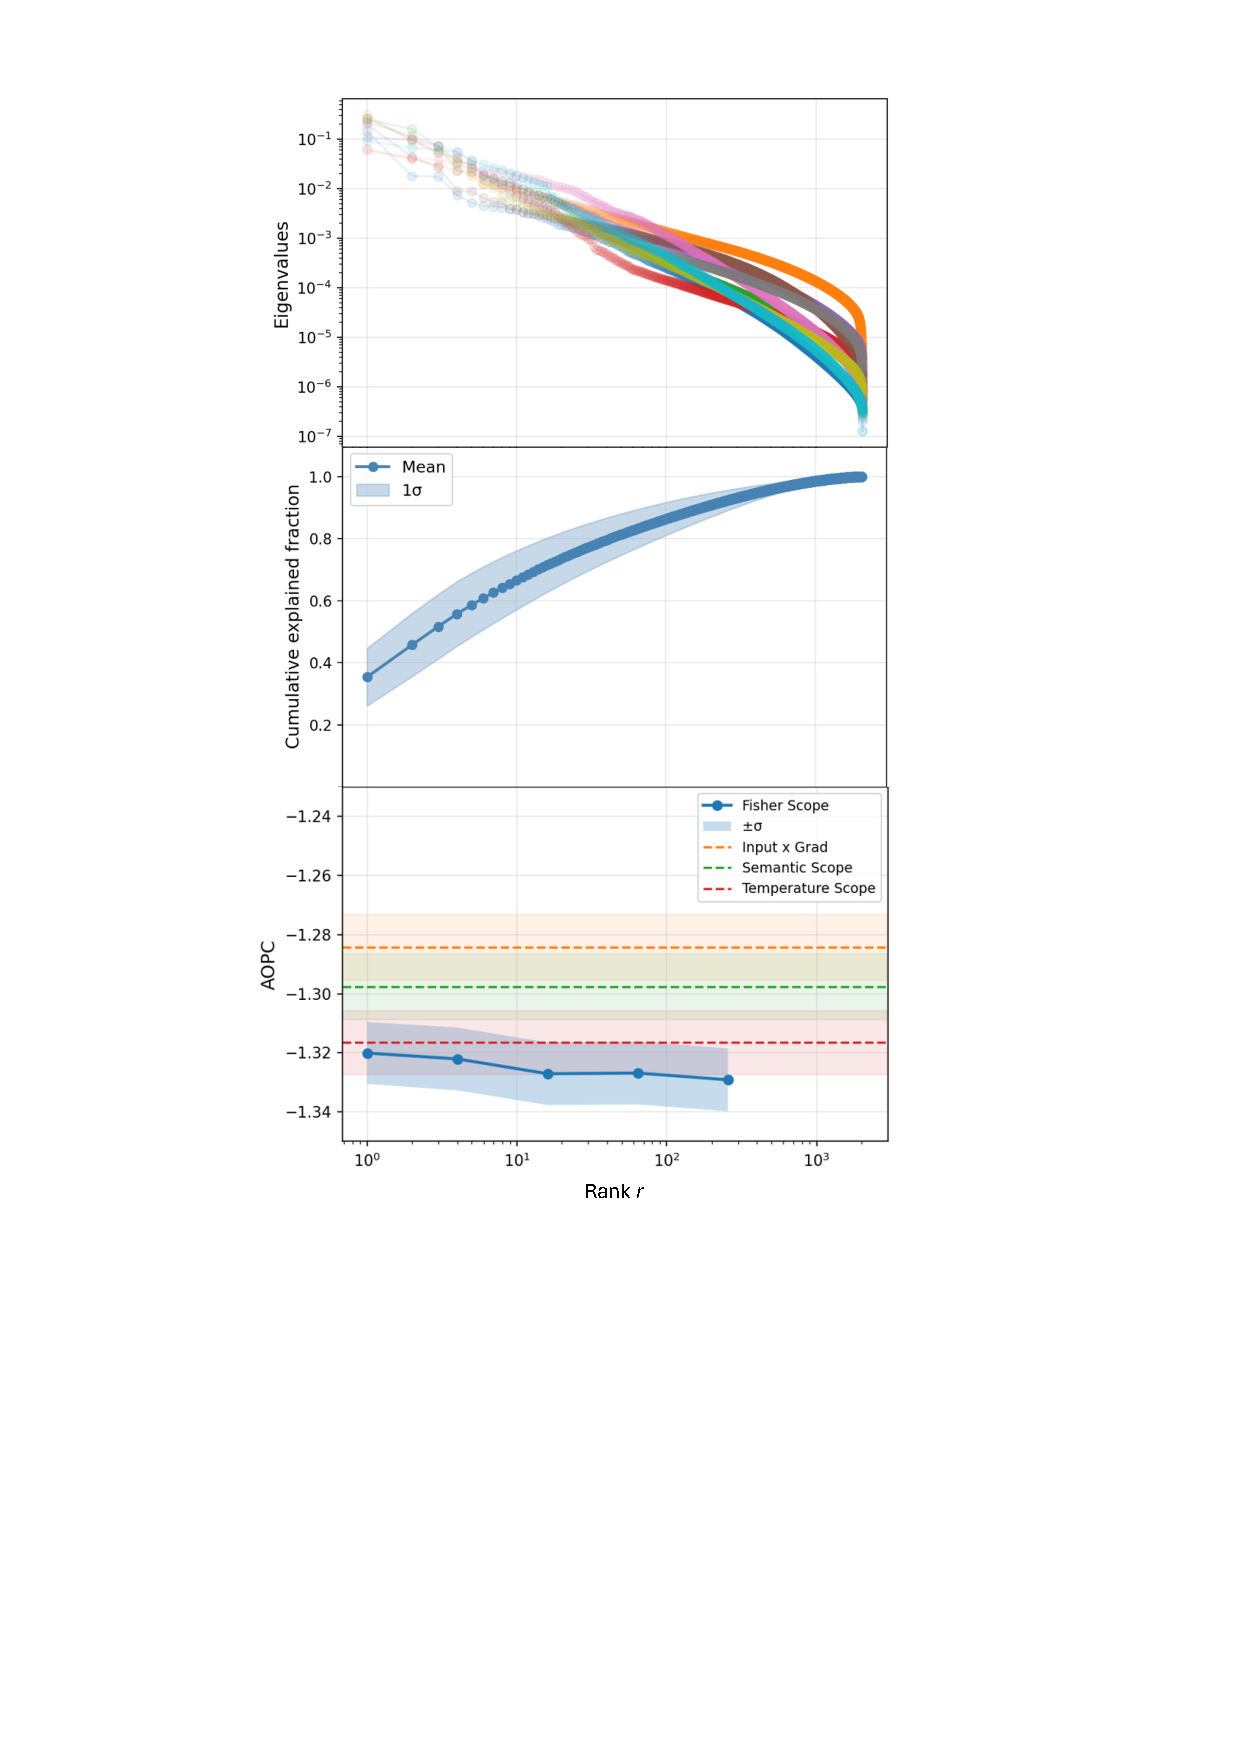
\includegraphics[width=0.9\columnwidth]{figures/fisher_ranks.pdf}
  \caption{Justification for the rank-1 approximation used in Fisher Scope, evaluated on LLaMA-3.2 1B and LAMBADA.
  \textbf{Top:} Eigenvalue spectrum of $\bm{F}$ across 10 prompts on a log-log scale, exhibiting a consistent power-law decay spanning 6 orders of magnitude.
  \textbf{Middle:} Mean cumulative explained variance $\sum_{i=1}^r \lambda_i / \mathrm{tr}(\bm{F})$ averaged over 1000 passages (shaded band: $\pm 1\sigma$); $\bm{u}_1$ alone accounts for $\approx$37\% of total sensitivity (1$\sigma$: 25--50\%).
  \textbf{Bottom:} AOPC as a function of rank $r \in \{1, 4, 16, 64, 256\}$, with baselines shown as dashed lines. Rank-1 Fisher Scope already outperforms Input $\times$ Gradient and Semantic Scope; increasing $r$ yields only marginal improvement at $r$-fold computational cost.}
  \label{fig:fisher_spectrum}
\end{figure}
The top panel shows the eigenvalue spectrum of $\bm{F}$ across 10 LAMBADA prompts on a log-log scale: a consistent power-law decay spanning 6 orders of magnitude, indicating that the leading eigenvalue dominates all subsequent ones.

The middle panel confirms this quantitatively via the cumulative explained variance $\sum_{i=1}^r \lambda_i / \mathrm{tr}(\bm{F})$, averaged over 1000 LAMBADA passages: 
at $r=1$ the mean explained fraction is already $\approx 37\%$, rising to $\approx 65\%$ by $r=10$ and approaching 1 only beyond $r \approx 1000$.

The bottom panel provides direct empirical justification, extending the LLaMA-3.2 1B results in \cref{tab:aupc}: rank-1 Fisher Scope ($r=1$) already outperforms Input $\times$ Gradient and Semantic Scope on LAMBADA, and matches Temperature Scope.
Increasing the rank to $r \in \{4, 16, 64, 256\}$ yields only marginal further gains in AOPC, while multiplying the computational cost by $r$.

Together, these results justify both the privileged status of $\bm{u}_1$ and the choice of $r=1$ in Fisher Scope.


\clearpage
\section*{NeurIPS Paper Checklist}



\begin{enumerate}

\item {\bf Claims}
    \item[] Question: Do the main claims made in the abstract and introduction accurately reflect the paper's contributions and scope?
    \item[] Answer: \answerYes{} % Replace by \answerYes{}, \answerNo{}, or \answerNA{}.
    \item[] Justification: The abstract and \cref{sec:methodology} clearly state the paper's contributions: a Jacobian-based framework for input--output attribution in LLMs, three concrete instantiations (Semantic Scope, Fisher Scope, and Temperature Scope), case studies, and a faithfulness evaluation on LAMBADA and IWSLT2017 across six LLMs (\cref{sec:evaluation}), with the significance claim supported by the paired tests in \cref{sec:paired_full}. Limitations and scope are discussed in the Limitations section.
    \item[] Guidelines:
    \begin{itemize}
        \item The answer \answerNA{} means that the abstract and introduction do not include the claims made in the paper.
        \item The abstract and/or introduction should clearly state the claims made, including the contributions made in the paper and important assumptions and limitations. A \answerNo{} or \answerNA{} answer to this question will not be perceived well by the reviewers. 
        \item The claims made should match theoretical and experimental results, and reflect how much the results can be expected to generalize to other settings. 
        \item It is fine to include aspirational goals as motivation as long as it is clear that these goals are not attained by the paper. 
    \end{itemize}

\item {\bf Limitations}
    \item[] Question: Does the paper discuss the limitations of the work performed by the authors?
    \item[] Answer: \answerYes{} % Replace by \answerYes{}, \answerNo{}, or \answerNA{}.
    \item[] Justification: The paper includes a dedicated Limitations section discussing these points.
    \item[] Guidelines:
    \begin{itemize}
        \item The answer \answerNA{} means that the paper has no limitation while the answer \answerNo{} means that the paper has limitations, but those are not discussed in the paper. 
        \item The authors are encouraged to create a separate ``Limitations'' section in their paper.
        \item The paper should point out any strong assumptions and how robust the results are to violations of these assumptions (e.g., independence assumptions, noiseless settings, model well-specification, asymptotic approximations only holding locally). The authors should reflect on how these assumptions might be violated in practice and what the implications would be.
        \item The authors should reflect on the scope of the claims made, e.g., if the approach was only tested on a few datasets or with a few runs. In general, empirical results often depend on implicit assumptions, which should be articulated.
        \item The authors should reflect on the factors that influence the performance of the approach. For example, a facial recognition algorithm may perform poorly when image resolution is low or images are taken in low lighting. Or a speech-to-text system might not be used reliably to provide closed captions for online lectures because it fails to handle technical jargon.
        \item The authors should discuss the computational efficiency of the proposed algorithms and how they scale with dataset size.
        \item If applicable, the authors should discuss possible limitations of their approach to address problems of privacy and fairness.
        \item While the authors might fear that complete honesty about limitations might be used by reviewers as grounds for rejection, a worse outcome might be that reviewers discover limitations that aren't acknowledged in the paper. The authors should use their best judgment and recognize that individual actions in favor of transparency play an important role in developing norms that preserve the integrity of the community. Reviewers will be specifically instructed to not penalize honesty concerning limitations.
    \end{itemize}

\item {\bf Theory assumptions and proofs}
    \item[] Question: For each theoretical result, does the paper provide the full set of assumptions and a complete (and correct) proof?
    \item[] Answer: \answerYes{} % Replace by \answerYes{}, \answerNo{}, or \answerNA{}.
    \item[] Justification: \cref{app:epsilon_perturbation,app:kl_second_order,app:fisher_total_information}

    \item[] Guidelines:
    \begin{itemize}
        \item The answer \answerNA{} means that the paper does not include theoretical results. 
        \item All the theorems, formulas, and proofs in the paper should be numbered and cross-referenced.
        \item All assumptions should be clearly stated or referenced in the statement of any theorems.
        \item The proofs can either appear in the main paper or the supplemental material, but if they appear in the supplemental material, the authors are encouraged to provide a short proof sketch to provide intuition. 
        \item Inversely, any informal proof provided in the core of the paper should be complemented by formal proofs provided in appendix or supplemental material.
        \item Theorems and Lemmas that the proof relies upon should be properly referenced. 
    \end{itemize}

    \item {\bf Experimental result reproducibility}
    \item[] Question: Does the paper fully disclose all the information needed to reproduce the main experimental results of the paper to the extent that it affects the main claims and/or conclusions of the paper (regardless of whether the code and data are provided or not)?
    \item[] Answer: \answerYes{} 
    \item[] Justification: \cref{sec:methodology,sec:evaluation} provide sufficient detail to reproduce all results.
    \item[] Guidelines:
    \begin{itemize}
        \item The answer \answerNA{} means that the paper does not include experiments.
        \item If the paper includes experiments, a \answerNo{} answer to this question will not be perceived well by the reviewers: Making the paper reproducible is important, regardless of whether the code and data are provided or not.
        \item If the contribution is a dataset and\slash or model, the authors should describe the steps taken to make their results reproducible or verifiable. 
        \item Depending on the contribution, reproducibility can be accomplished in various ways. For example, if the contribution is a novel architecture, describing the architecture fully might suffice, or if the contribution is a specific model and empirical evaluation, it may be necessary to either make it possible for others to replicate the model with the same dataset, or provide access to the model. In general. releasing code and data is often one good way to accomplish this, but reproducibility can also be provided via detailed instructions for how to replicate the results, access to a hosted model (e.g., in the case of a large language model), releasing of a model checkpoint, or other means that are appropriate to the research performed.
        \item While NeurIPS does not require releasing code, the conference does require all submissions to provide some reasonable avenue for reproducibility, which may depend on the nature of the contribution. For example
        \begin{enumerate}
            \item If the contribution is primarily a new algorithm, the paper should make it clear how to reproduce that algorithm.
            \item If the contribution is primarily a new model architecture, the paper should describe the architecture clearly and fully.
            \item If the contribution is a new model (e.g., a large language model), then there should either be a way to access this model for reproducing the results or a way to reproduce the model (e.g., with an open-source dataset or instructions for how to construct the dataset).
            \item We recognize that reproducibility may be tricky in some cases, in which case authors are welcome to describe the particular way they provide for reproducibility. In the case of closed-source models, it may be that access to the model is limited in some way (e.g., to registered users), but it should be possible for other researchers to have some path to reproducing or verifying the results.
        \end{enumerate}
    \end{itemize}


\item {\bf Open access to data and code}
    \item[] Question: Does the paper provide open access to the data and code, with sufficient instructions to faithfully reproduce the main experimental results, as described in supplemental material?
    \item[] Answer: \answerYes{} % Replace by \answerYes{}, \answerNo{}, or \answerNA{}.
    \item[] Justification: Our code is open-sourced at \url{https://github.com/AntonioLiu97/JacobianScopes}, and an interactive demo is hosted at \url{https://huggingface.co/spaces/Typony/JacobianScopes}. The three influence scores are given in closed form (\cref{sec:Semantic Scope,sec:fisher_scope,sec:Temperature Scope}), the benchmark datasets (LAMBADA and IWSLT2017) are publicly available, the base models (LLaMA-3.2, Qwen2.5, Gemma-3) are open-weight, and the evaluation protocol (AOPC) is described in full in \cref{sec:evaluation,sec:benchmark_details}.
    \item[] Guidelines:
    \begin{itemize}
        \item The answer \answerNA{} means that paper does not include experiments requiring code.
        \item Please see the NeurIPS code and data submission guidelines (\url{https://neurips.cc/public/guides/CodeSubmissionPolicy}) for more details.
        \item While we encourage the release of code and data, we understand that this might not be possible, so \answerNo{} is an acceptable answer. Papers cannot be rejected simply for not including code, unless this is central to the contribution (e.g., for a new open-source benchmark).
        \item The instructions should contain the exact command and environment needed to run to reproduce the results. See the NeurIPS code and data submission guidelines (\url{https://neurips.cc/public/guides/CodeSubmissionPolicy}) for more details.
        \item The authors should provide instructions on data access and preparation, including how to access the raw data, preprocessed data, intermediate data, and generated data, etc.
        \item The authors should provide scripts to reproduce all experimental results for the new proposed method and baselines. If only a subset of experiments are reproducible, they should state which ones are omitted from the script and why.
        \item At submission time, to preserve anonymity, the authors should release anonymized versions (if applicable).
        \item Providing as much information as possible in supplemental material (appended to the paper) is recommended, but including URLs to data and code is permitted.
    \end{itemize}


\item {\bf Experimental setting/details}
    \item[] Question: Does the paper specify all the training and test details (e.g., data splits, hyperparameters, how they were chosen, type of optimizer) necessary to understand the results?
    \item[] Answer: \answerYes{} % Replace by \answerYes{}, \answerNo{}, or \answerNA{}.
    \item[] Justification: Details regarding dataset and benchmark setup can be found in \cref{sec:evaluation,sec:benchmark_details}.
    \item[] Guidelines:
    \begin{itemize}
        \item The answer \answerNA{} means that the paper does not include experiments.
        \item The experimental setting should be presented in the core of the paper to a level of detail that is necessary to appreciate the results and make sense of them.
        \item The full details can be provided either with the code, in appendix, or as supplemental material.
    \end{itemize}

\item {\bf Experiment statistical significance}
    \item[] Question: Does the paper report error bars suitably and correctly defined or other appropriate information about the statistical significance of the experiments?
    \item[] Answer: \answerYes{} % Replace by \answerYes{}, \answerNo{}, or \answerNA{}.
    \item[] Justification: \Cref{sec:evaluation} reports mean AOPC over 1000 passages per model--dataset pair. \Cref{sec:paired_full} reports per-passage paired differences between the best Scope and the best baseline, with Student-$t$ 95\% confidence intervals and two-sided Wilcoxon signed-rank tests.
    \item[] Guidelines:
    \begin{itemize}
        \item The answer \answerNA{} means that the paper does not include experiments.
        \item The authors should answer \answerYes{} if the results are accompanied by error bars, confidence intervals, or statistical significance tests, at least for the experiments that support the main claims of the paper.
        \item The factors of variability that the error bars are capturing should be clearly stated (for example, train/test split, initialization, random drawing of some parameter, or overall run with given experimental conditions).
        \item The method for calculating the error bars should be explained (closed form formula, call to a library function, bootstrap, etc.)
        \item The assumptions made should be given (e.g., Normally distributed errors).
        \item It should be clear whether the error bar is the standard deviation or the standard error of the mean.
        \item It is OK to report 1-sigma error bars, but one should state it. The authors should preferably report a 2-sigma error bar than state that they have a 96\% CI, if the hypothesis of Normality of errors is not verified.
        \item For asymmetric distributions, the authors should be careful not to show in tables or figures symmetric error bars that would yield results that are out of range (e.g., negative error rates).
        \item If error bars are reported in tables or plots, the authors should explain in the text how they were calculated and reference the corresponding figures or tables in the text.
    \end{itemize}

\item {\bf Experiments compute resources}
    \item[] Question: For each experiment, does the paper provide sufficient information on the computer resources (type of compute workers, memory, time of execution) needed to reproduce the experiments?
    \item[] Answer: \answerYes{} % Replace by \answerYes{}, \answerNo{}, or \answerNA{}.
    \item[] Justification: We report the GPU type (NVIDIA RTX A4000) and representative forward/backward wall-clock times in the Limitations section.
    \item[] Guidelines:
    \begin{itemize}
        \item The answer \answerNA{} means that the paper does not include experiments.
        \item The paper should indicate the type of compute workers CPU or GPU, internal cluster, or cloud provider, including relevant memory and storage.
        \item The paper should provide the amount of compute required for each of the individual experimental runs as well as estimate the total compute. 
        \item The paper should disclose whether the full research project required more compute than the experiments reported in the paper (e.g., preliminary or failed experiments that didn't make it into the paper). 
    \end{itemize}
    
\item {\bf Code of ethics}
    \item[] Question: Does the research conducted in the paper conform, in every respect, with the NeurIPS Code of Ethics \url{https://neurips.cc/public/EthicsGuidelines}?
    \item[] Answer: \answerYes{} % Replace by \answerYes{}, \answerNo{}, or \answerNA{}.
    \item[] Justification: We follow the NeurIPS Code of Ethics.
    \item[] Guidelines:
    \begin{itemize}
        \item The answer \answerNA{} means that the authors have not reviewed the NeurIPS Code of Ethics.
        \item If the authors answer \answerNo, they should explain the special circumstances that require a deviation from the Code of Ethics.
        \item The authors should make sure to preserve anonymity (e.g., if there is a special consideration due to laws or regulations in their jurisdiction).
    \end{itemize}


\item {\bf Broader impacts}
    \item[] Question: Does the paper discuss both potential positive societal impacts and negative societal impacts of the work performed?
    \item[] Answer: \answerYes{} % Replace by \answerYes{}, \answerNo{}, or \answerNA{}.
    \item[] Justification: \cref{sec:Semantic Scope} and \cref{fig:causal attribution 2} in the main paper demonstrate how Semantic Scope can surface implicit political biases in LLMs, illustrating a direct application to model auditing and fairness analysis. We regard the negative risk as relatively indirect: Jacobian Scopes are a diagnostic tool that characterizes, but does not modify, model behaviour, and confer no additional control over the model itself.
    \item[] Guidelines:
    \begin{itemize}
        \item The answer \answerNA{} means that there is no societal impact of the work performed.
        \item If the authors answer \answerNA{} or \answerNo, they should explain why their work has no societal impact or why the paper does not address societal impact.
        \item Examples of negative societal impacts include potential malicious or unintended uses (e.g., disinformation, generating fake profiles, surveillance), fairness considerations (e.g., deployment of technologies that could make decisions that unfairly impact specific groups), privacy considerations, and security considerations.
        \item The conference expects that many papers will be foundational research and not tied to particular applications, let alone deployments. However, if there is a direct path to any negative applications, the authors should point it out. For example, it is legitimate to point out that an improvement in the quality of generative models could be used to generate Deepfakes for disinformation. On the other hand, it is not needed to point out that a generic algorithm for optimizing neural networks could enable people to train models that generate Deepfakes faster.
        \item The authors should consider possible harms that could arise when the technology is being used as intended and functioning correctly, harms that could arise when the technology is being used as intended but gives incorrect results, and harms following from (intentional or unintentional) misuse of the technology.
        \item If there are negative societal impacts, the authors could also discuss possible mitigation strategies (e.g., gated release of models, providing defenses in addition to attacks, mechanisms for monitoring misuse, mechanisms to monitor how a system learns from feedback over time, improving the efficiency and accessibility of ML).
    \end{itemize}
    
\item {\bf Safeguards}
    \item[] Question: Does the paper describe safeguards that have been put in place for responsible release of data or models that have a high risk for misuse (e.g., pre-trained language models, image generators, or scraped datasets)?
    \item[] Answer: \answerNA{} % Replace by \answerYes{}, \answerNo{}, or \answerNA{}.
    \item[] Justification: Our work does not pose such risks.
    \item[] Guidelines:
    \begin{itemize}
        \item The answer \answerNA{} means that the paper poses no such risks.
        \item Released models that have a high risk for misuse or dual-use should be released with necessary safeguards to allow for controlled use of the model, for example by requiring that users adhere to usage guidelines or restrictions to access the model or implementing safety filters. 
        \item Datasets that have been scraped from the Internet could pose safety risks. The authors should describe how they avoided releasing unsafe images.
        \item We recognize that providing effective safeguards is challenging, and many papers do not require this, but we encourage authors to take this into account and make a best faith effort.
    \end{itemize}

\item {\bf Licenses for existing assets}
    \item[] Question: Are the creators or original owners of assets (e.g., code, data, models), used in the paper, properly credited and are the license and terms of use explicitly mentioned and properly respected?
    \item[] Answer: \answerYes{} % Replace by \answerYes{}, \answerNo{}, or \answerNA{}.
    \item[] Justification: We cite the creators of the LLMs and datasets used throughout the paper.
    \item[] Guidelines:
    \begin{itemize}
        \item The answer \answerNA{} means that the paper does not use existing assets.
        \item The authors should cite the original paper that produced the code package or dataset.
        \item The authors should state which version of the asset is used and, if possible, include a URL.
        \item The name of the license (e.g., CC-BY 4.0) should be included for each asset.
        \item For scraped data from a particular source (e.g., website), the copyright and terms of service of that source should be provided.
        \item If assets are released, the license, copyright information, and terms of use in the package should be provided. For popular datasets, \url{paperswithcode.com/datasets} has curated licenses for some datasets. Their licensing guide can help determine the license of a dataset.
        \item For existing datasets that are re-packaged, both the original license and the license of the derived asset (if it has changed) should be provided.
        \item If this information is not available online, the authors are encouraged to reach out to the asset's creators.
    \end{itemize}

\item {\bf New assets}
    \item[] Question: Are new assets introduced in the paper well documented and is the documentation provided alongside the assets?
    \item[] Answer: \answerYes{} % Replace by \answerYes{}, \answerNo{}, or \answerNA{}.
    \item[] Justification: The only new asset is our open-source implementation of Jacobian Scopes, released with a README documenting installation, demonstration notebooks, and repository structure, together with a hosted interactive demo. No new datasets or models are introduced.
    \item[] Guidelines:
    \begin{itemize}
        \item The answer \answerNA{} means that the paper does not release new assets.
        \item Researchers should communicate the details of the dataset\slash code\slash model as part of their submissions via structured templates. This includes details about training, license, limitations, etc. 
        \item The paper should discuss whether and how consent was obtained from people whose asset is used.
        \item At submission time, remember to anonymize your assets (if applicable). You can either create an anonymized URL or include an anonymized zip file.
    \end{itemize}

\item {\bf Crowdsourcing and research with human subjects}
    \item[] Question: For crowdsourcing experiments and research with human subjects, does the paper include the full text of instructions given to participants and screenshots, if applicable, as well as details about compensation (if any)? 
    \item[] Answer: \answerNA{} % Replace by \answerYes{}, \answerNo{}, or \answerNA{}.
    \item[] Justification: Our work does not involve crowdsourcing or research with human subjects.
    \item[] Guidelines:
    \begin{itemize}
        \item The answer \answerNA{} means that the paper does not involve crowdsourcing nor research with human subjects.
        \item Including this information in the supplemental material is fine, but if the main contribution of the paper involves human subjects, then as much detail as possible should be included in the main paper. 
        \item According to the NeurIPS Code of Ethics, workers involved in data collection, curation, or other labor should be paid at least the minimum wage in the country of the data collector. 
    \end{itemize}

\item {\bf Institutional review board (IRB) approvals or equivalent for research with human subjects}
    \item[] Question: Does the paper describe potential risks incurred by study participants, whether such risks were disclosed to the subjects, and whether Institutional Review Board (IRB) approvals (or an equivalent approval/review based on the requirements of your country or institution) were obtained?
    \item[] Answer: \answerNA{} % Replace by \answerYes{}, \answerNo{}, or \answerNA{}.
    \item[] Justification: Our work does not involve crowdsourcing or research with human subjects.
    \item[] Guidelines:
    \begin{itemize}
        \item The answer \answerNA{} means that the paper does not involve crowdsourcing nor research with human subjects.
        \item Depending on the country in which research is conducted, IRB approval (or equivalent) may be required for any human subjects research. If you obtained IRB approval, you should clearly state this in the paper. 
        \item We recognize that the procedures for this may vary significantly between institutions and locations, and we expect authors to adhere to the NeurIPS Code of Ethics and the guidelines for their institution. 
        \item For initial submissions, do not include any information that would break anonymity (if applicable), such as the institution conducting the review.
    \end{itemize}

\item {\bf Declaration of LLM usage}
    \item[] Question: Does the paper describe the usage of LLMs if it is an important, original, or non-standard component of the core methods in this research? Note that if the LLM is used only for writing, editing, or formatting purposes and does \emph{not} impact the core methodology, scientific rigor, or originality of the research, declaration is not required.
    %this research? 
    \item[] Answer: \answerNA{} % Replace by \answerYes{}, \answerNo{}, or \answerNA{}.
    \item[] Justification: The core method development in our work does not involve LLMs as any important, original, or non-standard components.
    \item[] Guidelines:
    \begin{itemize}
        \item The answer \answerNA{} means that the core method development in this research does not involve LLMs as any important, original, or non-standard components.
        \item Please refer to our LLM policy in the NeurIPS handbook for what should or should not be described.
    \end{itemize}

\end{enumerate}
\end{document}
